
\index{stones}{$Q_1 \times P_0$ element}
\index{stones}{Compressible Flow}
\index{stones}{Mixed Formulation}
\index{stones}{Analytical Solution}
\index{stones}{Pressure Smoothing} 


\begin{mdframed}[backgroundcolor=red!5]
This work is part of the MSc thesis of T. Weir (2018).
\end{mdframed}

\Literature \cite{itki94,tagu07,lezh08,kilv10,lezh11,lizh13,hedg17,civj17}

\subsection*{The physics}

Let us start with some thermodynamics. Every material has an equation of state.
The equilibrium thermodynamic state of any material can
be constrained if any two state variables are specified.
Examples of state variables include
the pressure $p$ and specific volume $\nu = 1/\rho$, as well as the temperature $T$.

After linearisation, the density depends on temperature and pressure as follows:
\[
\rho(T,p) = \rho_0 \left((1 - \alpha(T-T_0) + \beta_T p \right)
\]
where $\alpha$ is the coefficient of thermal expansion, also called 
thermal expansivity: \index{stones}{thermal expansion}
\[
\alpha=-\frac{1}{\rho}\left( \frac{\partial \rho}{\partial T} \right)_p
\]
$\alpha$ is the percentage increase in volume of a material per degree of temperature increase; the
subscript $p$ means that the pressure is held fixed.

$\beta_T$ is the isothermal compressibility of the fluid, which is given by \index{stones}{compressibility}
\[
\beta_T = \frac{1}{K} = \frac{1}{\rho}\left( \frac{\partial \rho}{\partial P} \right)_T
\]
with $K$ the bulk modulus. \index{stones}{bulk modulus}
%aspect manual
Values of $\beta_T=10^{-12}-10^{-11}$ Pa$^{-1}$ are reasonable for Earth's mantle, with values decreasing by about a
factor of 5 between the shallow lithosphere and core-mantle boundary.
This is the percentage increase in density per unit change in pressure at constant temperature.
Both the coefficient of thermal expansion and the isothermal compressibility can be obtained
from the equation of state.

The full set of equations we wish to solve is given by

\begin{eqnarray}
-\nabla \cdot \left[2\eta \dot{\bm \epsilon}^d({\bm v}) \right] + \nabla p &=& \rho_0 \left((1 - \alpha(T-T_0) + \beta_T p \right) {\bm g} \quad\quad \textrm{in $\Omega$}  \label{eq:stokes-1} \\
\nabla \cdot {\bm v} + \frac{1}{\rho} {\bm v} \cdot {\bm \nabla}\rho&=&0 \quad\quad  \textrm{in $\Omega$}   \label{eq:stokes-2} \\
\rho C_p \left(\frac{\partial T}{\partial t} + \bm v\cdot\nabla T\right) - \nabla\cdot k\nabla T   &=& 
  \rho H  +  2\eta \dot{\bm \epsilon}^d : \dot{\bm \epsilon}^d    +\alpha T \left( \frac{\partial p}{\partial t}+  \bm v \cdot \nabla p \right) 
\quad\quad   \textrm{in $\Omega$},
  \label{eq:temperature}
\end{eqnarray}

Note that this presupposes that the density is not zero anywhere in the domain.


\subsection*{The numerics}

We use a mixed formulation and therefore  
keep both velocity and pressure as unknowns. We end up having to solve 
the following system:
\[
\left(
\begin{array}{cc}
\K & \G+\W \\ \G^T+\Z & 0 
\end{array}
\right)
\cdot
\left(
\begin{array}{c}
{\cal V} \\ {\cal P}
\end{array}
\right)
=
\left(
\begin{array}{c}
 f \\ h
\end{array}
\right)
\quad\quad
{\rm or,}
\quad\quad
\A \cdot X = rhs
\]
Where $\K$ is the stiffness matrix, $\G$ is the discrete gradient operator, 
$\G^T$ is the discrete divergence operator, ${\cal V}$ the velocity vector, 
${\cal P}$ the pressure vector.
Note that the term $\Z{\cal V}$ derives from term ${\bm v} \cdot {\bm \nabla} \rho$ in the continuity equation. 

As perfectly explained in the step 32 of deal.ii\footnote{https://www.dealii.org/9.0.0/doxygen/deal.II/step\_32.html},
we need to scale the $\G$ term since it is many orders of magnitude smaller than $\K$, which introduces large inaccuracies in the solving process to the point that the solution is nonsensical. This scaling coefficient is $\eta/L$. After building the $\G$ block, it is then scaled as follows: $\G'=\frac{\eta}{L}\G$ so that we now solve 

\[
\left(
\begin{array}{cc}
\K & \G'+\W \\ \G'^T+\Z & 0 
\end{array}
\right)
\cdot
\left(
\begin{array}{c}
{\cal V} \\ {\cal P}'
\end{array}
\right)
=
\left(
\begin{array}{c}
 f \\ h
\end{array}
\right)
\]
After the solve phase, we recover the real pressure with ${\cal P}=\frac{\eta}{L}{\cal P}'$.

{\color{red} adapt notes since I should scale $\W$ and $\Z$ too}.
{\color{red} $h$ should be caled too !!!!!!!!!!!!!!!} 

Each block $\K$, $\G$ , $\Z$ and vectors $f$ and $h$ are built separately 
in the code and assembled into 
the matrix $\A$ and vector $rhs$ afterwards. $\A$ and $rhs$ are then passed to the solver. 
We will see later that there are alternatives to solve this approach which do not require to 
build the full Stokes matrix $\A$. 

{\bf Remark 1}: the terms $\Z {\cal V}$ and $\W {\cal P}$ are 
often put in the rhs (i.e. added to $h$) so that 
the matrix $\A$ retains the same structure as in the incompressible case. This is indeed 
how it is implemented in ASPECT, see also appendix A of \cite{lezh08}. This however requires more work since the rhs depends 
on the solution and some form of iterations is needed. 

{\bf Remark 2}: Very often the adiabatic heating term  
$\alpha T \left( \bm v \cdot \nabla p \right)$ is simplified as follows:
%aspect manual
If you assume the vertical component of the gradient of the dynamic pressure to be small compared to the
gradient of the total pressure (in other words, the gradient is dominated by the gradient of the hydrostatic
pressure), then $-\rho {\bm g} \simeq {\bm \nabla}p$ and then 
$\alpha T \left( \bm v \cdot \nabla p \right) \simeq  -\alpha\rho T {\bm v}\cdot{\bm g}$. We will however 
not be using this approximation in what follows.



We have already established that
\[
\vec{\tau} = {\bm C}_\eta {\bm B} V
\]


The following measurements are carried out:
\begin{itemize}
\item The root mean square velocity ({\tt vrms}):
\[
v_{rms} = \sqrt{\frac{1}{V}\int_V v^2 dV   }
\]
\item The average temperature ({\tt Tavrg}):
\[
<T>=\frac{1}{V}\int_V T dV
\]
\item The total mass ({\tt mass}):
\[
M=\int_V \rho dV 
\]
\item The Nusselt number ({\tt Nu}):
\[
Nu=-\frac{1}{Lx}\frac{1}{\Delta T} \int_0^{L_x} \frac{\partial T(x,y=L_y)}{\partial y} dx
\]
\item The kinetic energy ({\tt EK}):
\[
E_K=\int_V \frac{1}{2}\rho v^2 dV
\]
\item The work done against gravity 
\[
<W>=-\int_V \rho g_y v_y dV
\]
\item The total viscous dissipation ({\tt visc\_diss})
\[
<\Phi>=\int \Phi dV =\frac{1}{V}\int 2 \eta \dot{\bm \varepsilon}:\dot{\bm \varepsilon} dV 
\]
\item The gravitational potential energy ({\tt EG})
\[
E_G = \int_V \rho g_y (L_y-y) dV
\]
\item The internal thermal energy ({\tt ET})
\[
E_T = \int_V \rho_{(0)} C_p T dV
\]

{\bf Remark 3:} Measuring the total mass can be misleading: indeed because $\rho=\rho_0(1-\alpha T)$, then 
measuring the total mass amounts to measuring a constant minus the volume-integrated temperature, and there is 
no reason why the latter should be zero, so that there is no reason why the total mass should be zero...!

\end{itemize}




\subsection*{The experimental setup}

The setup is as follows: the domain is $Lx=Ly=3000$km. Free slip boundary conditions are imposed on all four sides. 
The initial temperature is given by:
\[
T(x,y) = \left(  \frac{L_y-y}{Ly} - 0.01\cos(\frac{\pi x}{L_x}) \sin(\frac{\pi y}{Ly}) \right) \Delta T + T_{surf}
\]
with $\Delta T=4000$K, $T_{surf}=T_0=273.15$K. The temperature is set to $\Delta T + T_{surf}$ at the bottom and $T_{surf}$ at the top.
We also set $k=3$, $C_p=1250$, $|g|=10$, $\rho_0=3000$ and we keep the Rayleigh number $Ra$ and dissipation number $Di$ as input parameters:
\[
Ra=\frac{\alpha g \Delta T L^3 \rho_0^2 C_p}{\eta k}
\quad\quad
Di=\frac{\alpha g L}{C_p}
\]
From the second equation we get $\alpha=\frac{Di C_p}{g L}$, which we can insert in the first one:
\[
Ra=\frac{Di C_p^2 \Delta T L^2 \rho_0^2 }{\eta k}
\quad\quad
{\rm or,}
\quad\quad
\eta=
\frac{Di C_p^2 \Delta T L^2 \rho_0^2 }{Ra \; k  }
\]
For instance, for $Ra=10^4$ and $Di=0.75$, we obtain $\alpha\simeq 3\cdot 10^{-5}$ and $\eta\simeq 10^{25}$ 
which are quite reasonable values. 


\subsection*{Scaling}

Following \cite{kilv10}, we non-dimensionalize the equations using the reference values
for density $\rho_r$, thermal expansivity $\alpha_r$, 
temperature contrast $\Delta T_r$ ({\tt refTemp}),
thermal conductivity $k_r$, heat capacity $C_p$,  
depth of the fluid layer $L$ and viscosity $\eta_r$. The
non-dimensionalization for velocity, $u_r$ , pressure $p_r$ and time, $t_r$ become
\[
u_r = \frac{k_r}{\rho_r C_p L} \quad ({\tt refvel})
\]
\[
p_r=\frac{\eta_r k_r}{\rho_r C_p L^2}\quad  ({\tt refpress})
\]
\[
t_r=\frac{\rho_r C_p L^2}{k_r} \quad ({\tt reftime})
\]

In the case of the setup described hereabove, and when choosing 
$Ra=10^4$ and $Di=0.5$, we get:
\begin{verbatim}
alphaT 2.083333e-05 
eta 8.437500e+24 
reftime 1.125000e+19 
refvel 2.666667e-13 
refPress 7.500000e+05 
\end{verbatim}



%-------------------------------------------
\subsection*{Conservation of energy 1}



\subsubsection*{under BA and EBA approximations}

Following \cite{lezh08}, we take the dot product of the momentum equation with the velocity ${\bm v}$ and integrate over the whole volume\footnote{Check: this is akin to looking at the power, force*velocity,  says Arie}:
\[
\int_V  \left[ -\nabla \cdot {\bm \tau}  + {\bm \nabla} p \right] \cdot {\bm v} dV  = \int_V  \rho {\bm g} \cdot {\bm v}dV
\]
or, 
\[
-\int_V (\nabla \cdot {\bm \tau})\cdot {\bm v} dV +\int_V   {\bm \nabla} p \cdot {\bm v} dV  = \int_V  \rho {\bm g} \cdot {\bm v}dV
\]
Let us look at each block separately:
\[
-\int_V (\nabla \cdot {\bm \tau})\cdot {\bm v} dV 
=-\int_S  {\bm \tau} \underbrace{{\bm v}\cdot {\bm n}}_{=0 \; (b.c.)} dS + \int_V {\bm \tau}:{\bm \nabla}{\bm v} dV 
= \int_V {\bm \tau} : \dot{\bm \varepsilon} dV 
= \int_V \Phi  dV 
\]
which is the volume integral of the shear heating. Then,
\[
\int_V {\bm \nabla} p \cdot {\bm v} dV  =
\int_S p \underbrace{{\bm v}\cdot {\bm n}}_{=0 \; (b.c.)} dS - \int_V \underbrace{{\bm \nabla}\cdot{\bm v}}_{=0 \; (incomp.)} \; p dV = 0 
\]
which is then zero in the case of an incompressible flow. 
And finally
\[
\int_V \rho {\bm g} \cdot {\bm v} dV = W
\]
which is the work against gravity. \index{stones}{work against gravity} 

Conclusion for an {\it incompressible} fluid: we should have
\begin{equation}
\int_V \Phi  dV 
=
\int_V \rho {\bm g} \cdot {\bm v} dV 
\label{ba001}
\end{equation}
This formula is hugely problematic: indeed, the term $\rho$ in the rhs is the full density. We know 
that to the value of $\rho_0$ corresponds a lithostatic pressure gradient $p_L=\rho_0 g y$. In this case one can write $\rho = \rho_0 + \rho'$ and $p=p_L + p'$
so that we also have 
\[
\int_V  \left[ -\nabla \cdot {\bm \tau}  + {\bm \nabla} p' \right] \cdot {\bm v} dV  = \int_V  \rho' {\bm g} \cdot {\bm v}dV
\]
which will ultimately yield 
\begin{equation}
\int_V \Phi  dV 
=
\int_V \rho' {\bm g} \cdot {\bm v} dV 
=
\int_V (\rho-\rho_0) {\bm g} \cdot {\bm v} dV 
\label{ba002}
\end{equation}
Obviously Eqs.(\ref{ba001}) and (\ref{ba002}) cannot be true at the same time.
The problem comes from the nature of the (E)BA approximation: $\rho=\rho_0$ in the mass conservation equation
but it is not constant in the momentum conservation equation, which is of course inconsistent. Since the mass 
conservation equation is ${\bm \nabla}\cdot{\bm v}=0$ under this approximation then the term 
$\int_V {\bm \nabla} p \cdot {\bm v} dV$ is always zero for any pressure (full pressure $p$, or overpressure $p-p_L$), 
hence the paradox. This paradox will be lifted when a consistent set of equations will be used (compressible formulation).
On a practical note, Eqs.(\ref{ba001}) is not verified by the code, while (\ref{ba002}) is.   

In the end:
\begin{equation}
\boxed{
\underbrace{\int_V \Phi  dV }_{\tt visc\_diss}
=
\underbrace{\int_V (\rho-\rho_0) {\bm g} \cdot {\bm v} dV }_{\tt work\_grav}
}
\label{ba003}
\end{equation}


\subsubsection*{under no  approximation at all}

\begin{eqnarray}
\int_V {\bm \nabla} p \cdot {\bm v} dV  
&=& \int_S p \underbrace{{\bm v}\cdot {\bm n}}_{=0 \; (b.c.)} dS - \int_V {\bm \nabla}\cdot{\bm v} \; p dV = 0  \\
&=&  \int_V \frac{1}{\rho} {\bm v} \cdot {\bm \nabla} \rho \; p dV = 0  \\
\end{eqnarray}

{\color{red} ToDo}:see section 3 of \cite{lezh08} where this is carried out with the Adams-Williamson eos.


\subsection*{Conservation of energy 2}
Also, following the Reynold's transport theorem \cite{malvern},p210, we have for a property $A$ (per unit mass)
\[
\frac{d}{dt} \int_V A \rho dV = \int_V \frac{\partial }{\partial t} (A\rho) dV + \int_S A \rho {\bm v}\cdot {\bm n} dS
\]
Let us apply to this to $A=C_p T$ and compute the time derivative of the internal energy:
\begin{eqnarray}
\frac{d}{dt} \int_V \rho C_p T dV 
&=& \int_V \frac{\partial }{\partial t} (\rho C_p T ) dV + \int_S A \rho \underbrace{{\bm v}\cdot {\bm n}}_{=0 \; (b.c.)} dS 
= \underbrace{\int_V C_p T \frac{\partial \rho}{\partial t} dV}_{I} 
+ \underbrace{\int_V \rho C_p \frac{\partial T}{\partial t}  dV }_{II}
\end{eqnarray}

In order to expand $I$, the mass conservation equation will be used, while the heat transport equation 
will be used for $II$:

\begin{eqnarray}
I= \int_V C_p T \frac{\partial \rho}{\partial t} dV
&=& 
- \int_V C_p T {\bm \nabla} \cdot (\rho {\bm v}) dV
=
-\int_V C_p T \rho \underbrace{{\bm v} \cdot {\bm n}}_{=0 \; (b.c.)} dS +  \int_V \rho C_p  {\bm \nabla}  T \cdot {\bm v} dV
\\
II=\int_V \rho C_p \frac{\partial T}{\partial t}  dV
&=&  
 \int_V \left[ -\rho C_p {\bm v}\cdot {\bm \nabla}T +{\bm \nabla}\cdot k {\bm \nabla} T + \rho H  + \Phi    +\alpha T \left( \frac{\partial p}{\partial t}+  \bm v \cdot {\bm \nabla} p \right) \right]  dV \\ 
&=& 
 \int_V \left[ -\rho C_p {\bm v}\cdot {\bm \nabla}T 
+ \rho H  + \Phi    +\alpha T \left( \frac{\partial p}{\partial t}+  \bm v \cdot {\bm \nabla} p \right) \right]  dV 
+ \int_V {\bm \nabla}\cdot k {\bm \nabla} T dV \\ 
&=& 
 \int_V \left[ -\rho C_p {\bm v}\cdot {\bm \nabla}T 
+ \rho H  + \Phi    +\alpha T \left( \frac{\partial p}{\partial t}+  \bm v \cdot {\bm \nabla} p \right) \right]  dV 
+ \int_S  k {\bm \nabla} T \cdot {\bm n}  dS \\ 
&=& 
 \int_V \left[ -\rho C_p {\bm v}\cdot {\bm \nabla}T 
+ \rho H  + \Phi    +\alpha T \left( \frac{\partial p}{\partial t}+  \bm v \cdot {\bm \nabla} p \right) \right]  dV 
- \int_S  {\bm q} \cdot {\bm n}  dS \label{ba004}
\end{eqnarray}

Finally:

\begin{eqnarray}
I+II=\frac{d}{dt} \underbrace{\int_V \rho C_p T dV }_{\tt ET}
 &=& 
 \int_V \left[ 
 \rho H  + \Phi    +\alpha T \left( \frac{\partial p}{\partial t}+  \bm v \cdot {\bm \nabla} p \right) \right]  dV 
- \int_S  {\bm q} \cdot {\bm n}  dS \\ 
 &=& 
 \int_V \rho H dV 
+\underbrace{\int_V \Phi  dV}_{\tt visc\_diss}  
+\underbrace{\int_V \alpha T \frac{\partial p}{\partial t} dV}_{\tt extra}
+\underbrace{\int_V \alpha T \bm v \cdot {\bm \nabla} p  dV}_{\tt adiab\_heating} 
- \underbrace{\int_S  {\bm q} \cdot {\bm n}  dS}_{\tt heatflux\_boundary} \label{ba005}
\end{eqnarray}

This was of course needlessly complicated as the term $\partial \rho/\partial t$ is always 
taken to be zero, so that $I=0$ automatically. The mass conservation equation is then 
simply ${\bm \nabla}\cdot (\rho {\bm v})=0$. Then it follows that 
\begin{eqnarray}
0&=& \int_V C_p T {\bm \nabla} \cdot (\rho {\bm v}) dV
=
-\int_V C_p T \rho \underbrace{{\bm v} \cdot {\bm n}}_{=0 \; (b.c.)} dS +  \int_V \rho C_p  {\bm \nabla}  T \cdot {\bm v} dV \\
&=&  \int_V \rho C_p  {\bm \nabla}  T \cdot {\bm v} dV 
\end{eqnarray}
so that the same term in Eq.(\ref{ba004}) vanishes too, and then Eq.(\ref{ba005}) is always valid, although one should be careful when computing $E_T$ in the BA and EBA cases as it should use $\rho_0$ and not $\rho$.


%-------------------------------------------
\subsection*{The problem of the onset of convection}

[wiki] In geophysics, the Rayleigh number is of fundamental importance: it indicates the presence and strength of convection within a fluid body such as the Earth's mantle. The mantle is a solid that behaves as a fluid over geological time scales.

 The Rayleigh number essentially is an indicator of the type of heat transport mechanism. At low Rayleigh numbers conduction processes dominate over convection ones. At high Rayleigh numbers it is the other way around. There is a so-called critical value of the number with delineates the transition from one regime to the other. 

This problem has been studied and approached both theoretically and numerically \cite[e.g.]{tusc} and it was found that
the critical Rayleigh number $Ra_c$ is 
\[
Ra_c=(27/4)\pi^4 \simeq 657.5
\]
in setups similar to ours.


\vspace{3cm}



{\color{red} VERY BIG PROBLEM}

The temperature setup is built as follows: $T_{surf}$ is prescribed at the top, 
$T_{surf}+\Delta T$ is prescribed at the bottom. The initial temperature profile is linear between these two values. 
In the case of BA, the actual value of $T_{surf}$ is of no consequence. However, for the EBA the full temperature is present in the adiabatic heating term on the rhs of the hte, and the value of $T_{surf}$ will therefore influence the solution greatly. This is very problematic as there is no real way to arrive at the surface temperature from the King paper. On top of this, the density uses a reference temperature $T_0$ which too will influence the solution without being present in the controlling $Ra$ and $Di$ numbers!!

In light thereof, it will be very difficult to recover the values of King et al for EBA!

\vspace{3cm}


Relevant literature: \cite{besg92,itki94,tagu07,lezh08,kilv10,lezh11,lizh13,hedg17}

%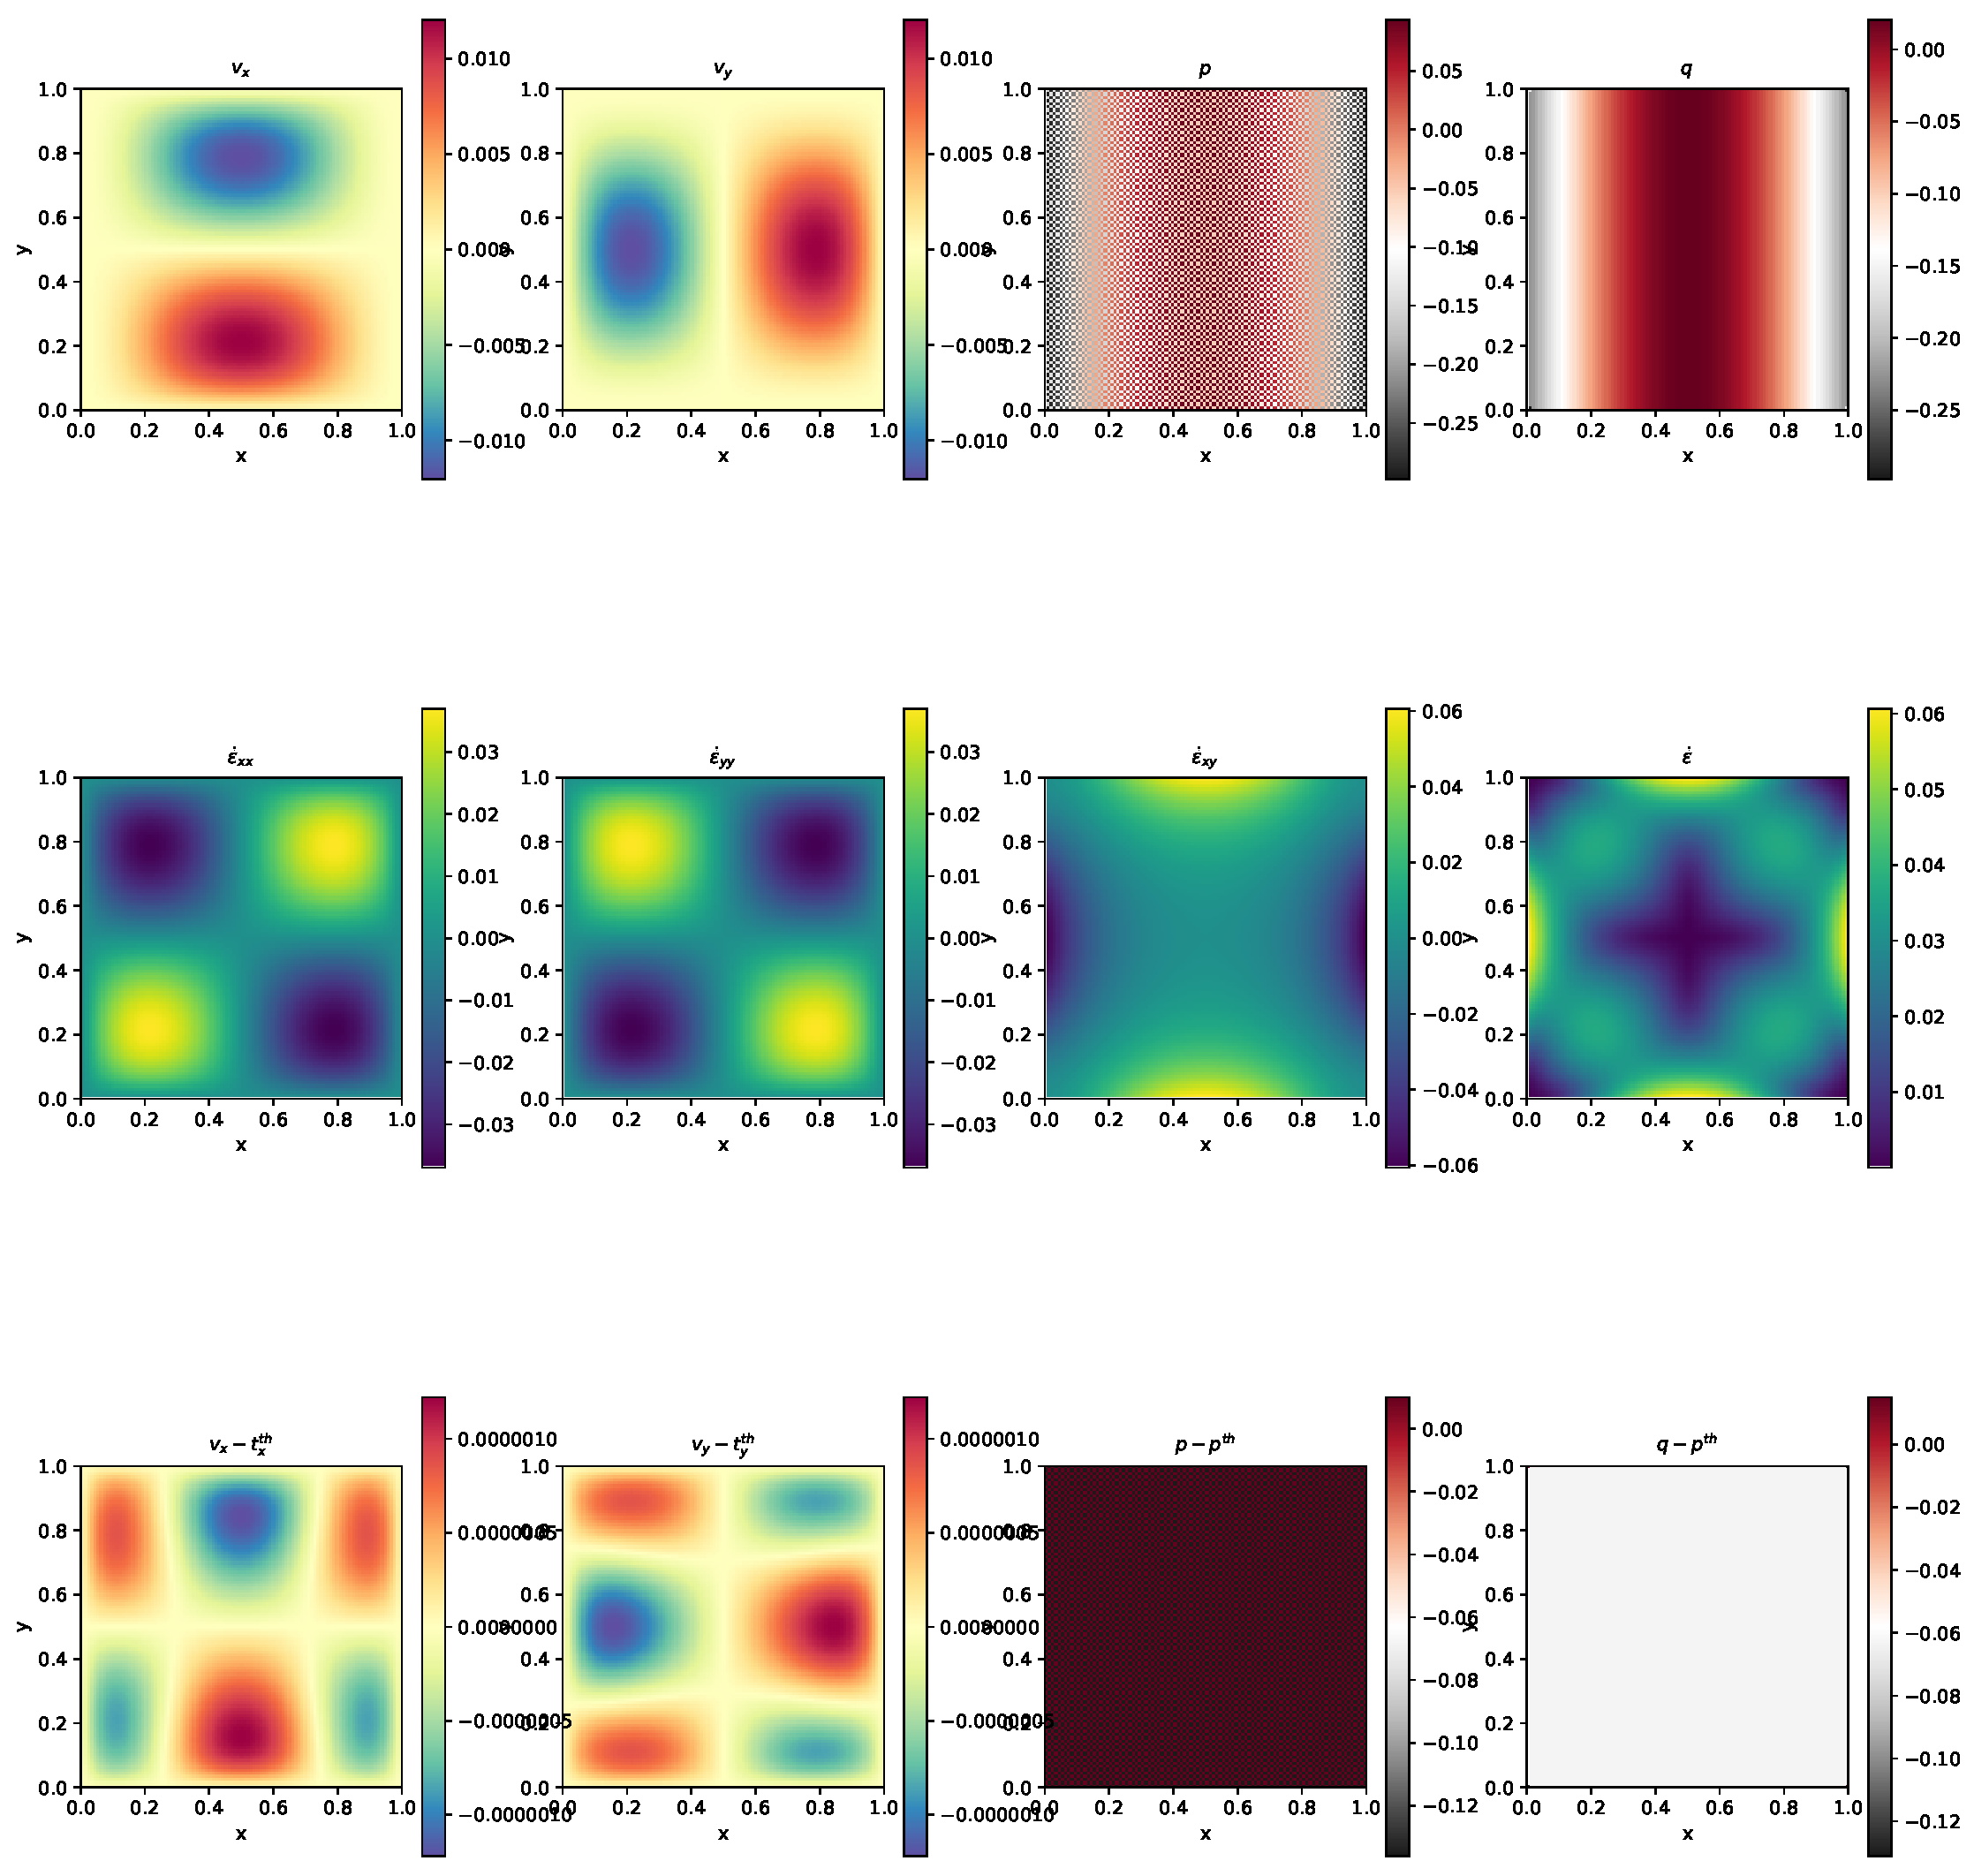
\includegraphics[width=16cm]{python_codes/fieldstone_saddlepoint/solution.pdf}

ToDo: 
\begin{itemize}
\item heat flux is at the moment elemental, so Nusselt and heat flux on boundaries measurements not as accurate as could be.
\item implement steady state detection
\item do $Ra=10^5$ and $Ra=10^6$
\item velocity average at surface
\item non dimensional heat flux at corners \cite{blbc89} 
\item depth-dependent viscosity (case 2 of \cite{blbc89})
\end{itemize}

\newpage
%-------------------------------------------------------
\subsection*{results - BA - $Ra=10^4$}

These results were obtained with a 64x64 resolution, and CFL number of 1. Steady state was reached 
after about 1250 timesteps.

\begin{center}
(a)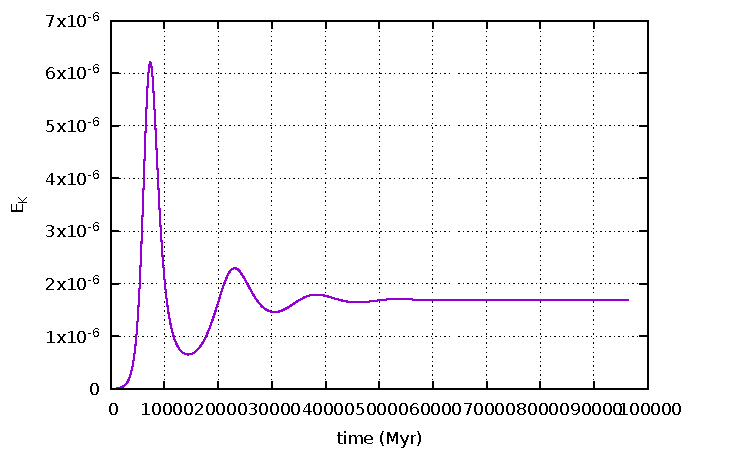
\includegraphics[width=4.5cm]{python_codes/fieldstone_24/BA_104/EK}
(b)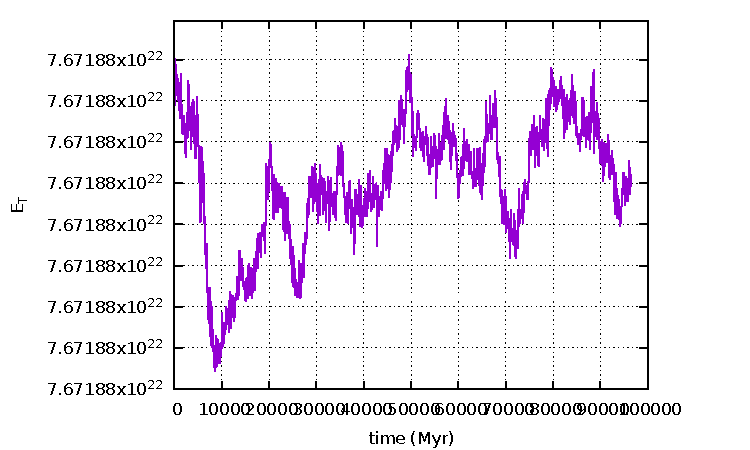
\includegraphics[width=4.5cm]{python_codes/fieldstone_24/BA_104/ET}
(c)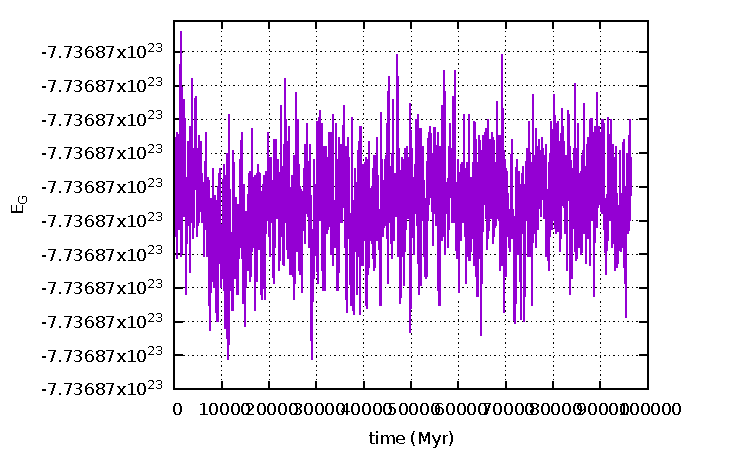
\includegraphics[width=4.5cm]{python_codes/fieldstone_24/BA_104/EG}\\
(d)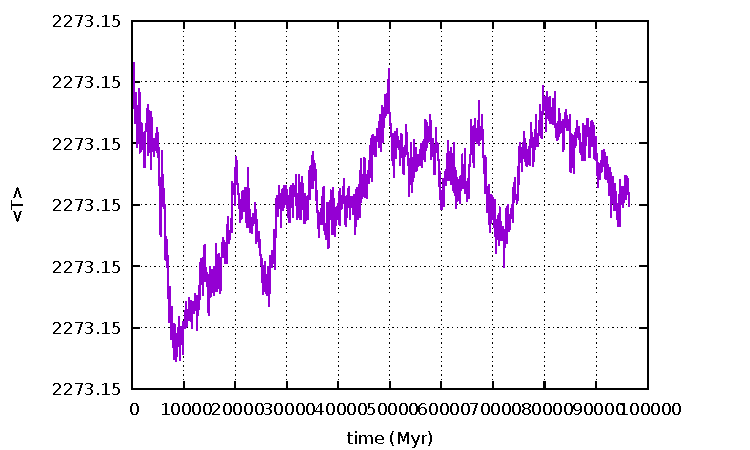
\includegraphics[width=4.5cm]{python_codes/fieldstone_24/BA_104/Tavrg}
(e)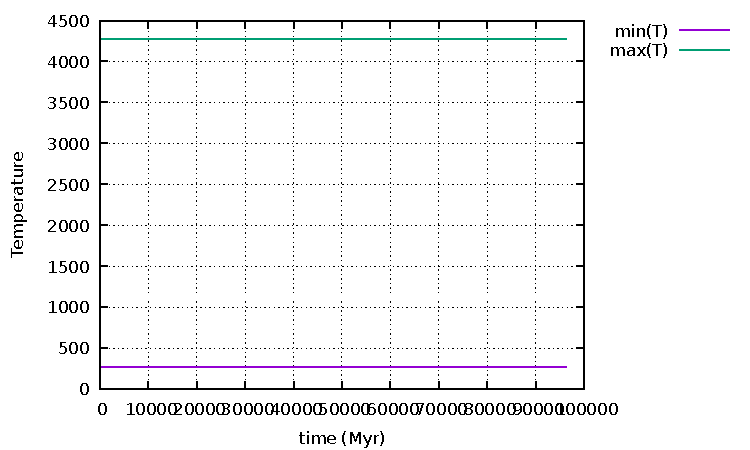
\includegraphics[width=4.5cm]{python_codes/fieldstone_24/BA_104/T_stats}
(f)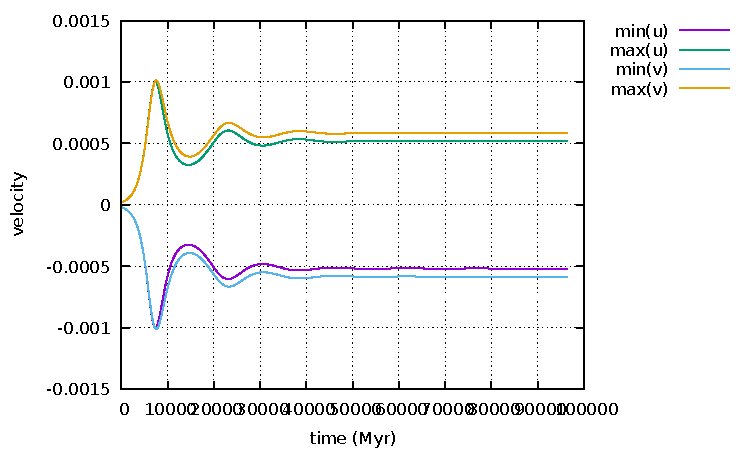
\includegraphics[width=4.5cm]{python_codes/fieldstone_24/BA_104/vel_stats}\\
(g)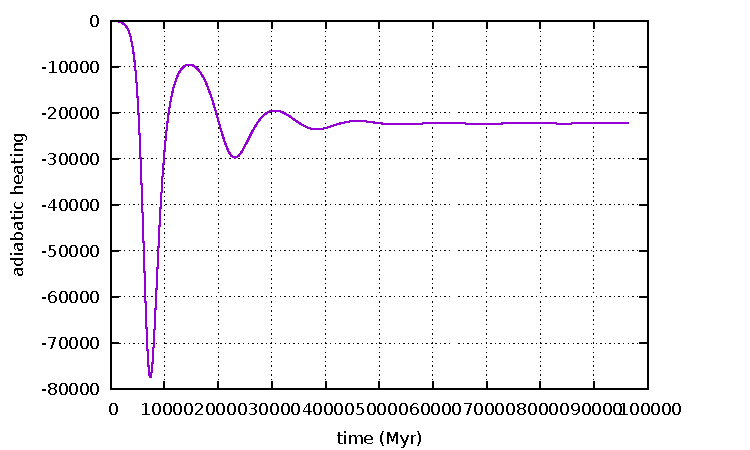
\includegraphics[width=4.5cm]{python_codes/fieldstone_24/BA_104/adiabatic_heating}
(h)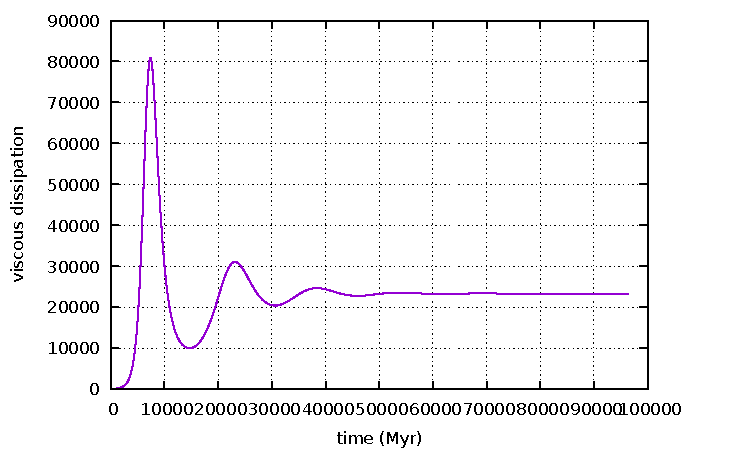
\includegraphics[width=4.5cm]{python_codes/fieldstone_24/BA_104/viscous_dissipation}
(i)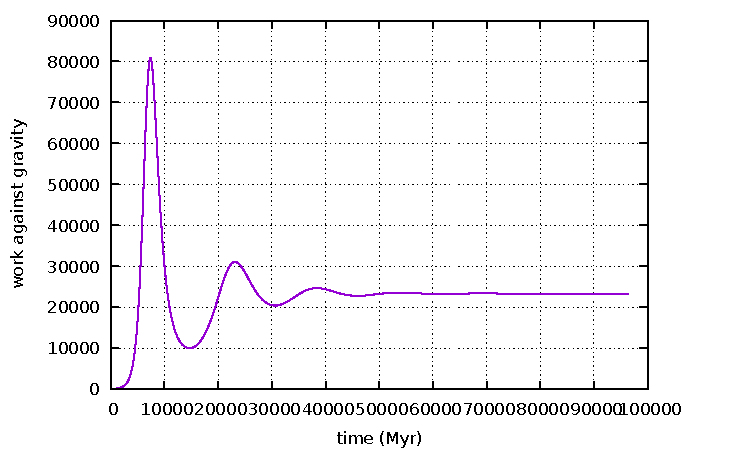
\includegraphics[width=4.5cm]{python_codes/fieldstone_24/BA_104/work_grav}\\
(j)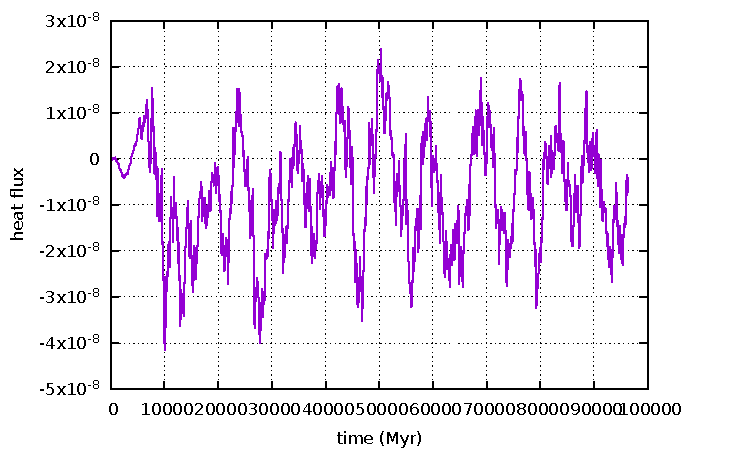
\includegraphics[width=4.5cm]{python_codes/fieldstone_24/BA_104/heat_flux}
(k)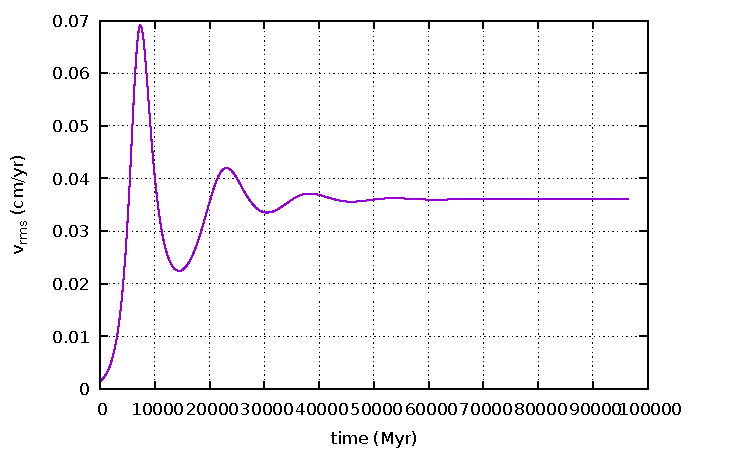
\includegraphics[width=4.5cm]{python_codes/fieldstone_24/BA_104/vrms}
(l)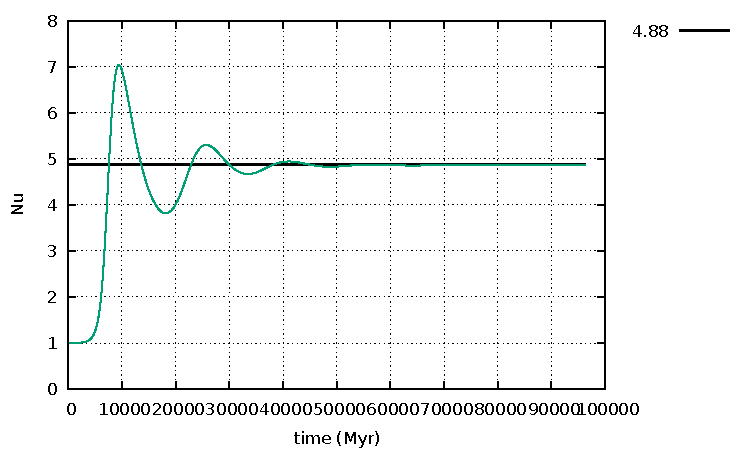
\includegraphics[width=4.5cm]{python_codes/fieldstone_24/BA_104/Nu}\\
(l)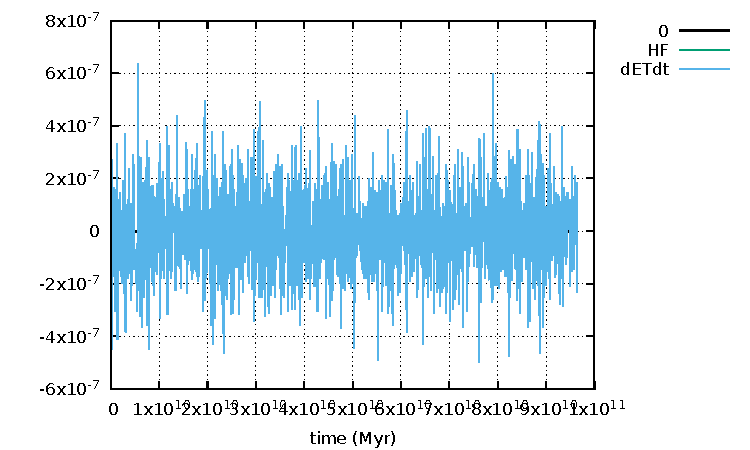
\includegraphics[width=7cm]{python_codes/fieldstone_24/BA_104/conservation1}
(m)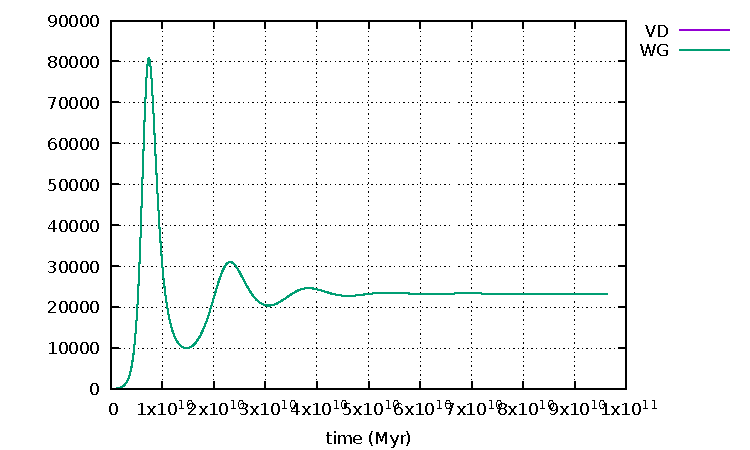
\includegraphics[width=7cm]{python_codes/fieldstone_24/BA_104/conservation2}\\
AH: adiabatic heating, VD: viscous dissipation, HF: heat flux, WG: work against gravity
\end{center}

Eq.(\ref{ba005}) is verified by (l) and Eq.(\ref{ba003}) is verified by (m).


\newpage
\begin{center}
(a)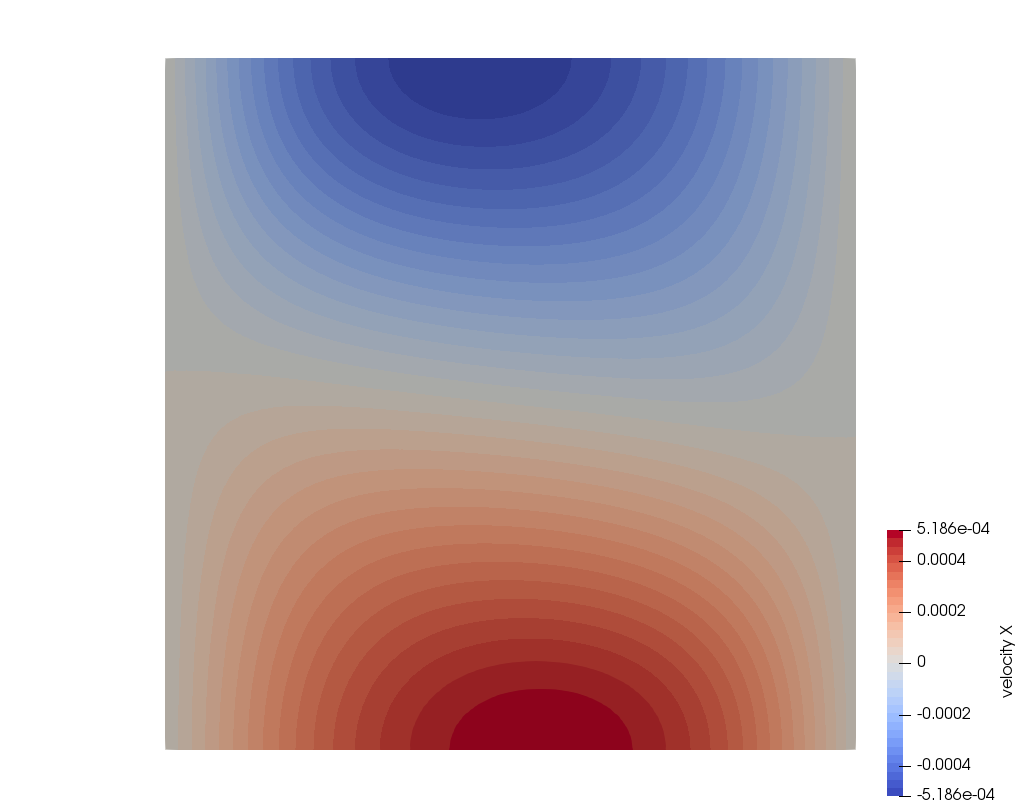
\includegraphics[width=4.5cm]{python_codes/fieldstone_24/BA_104/u.png}
(b)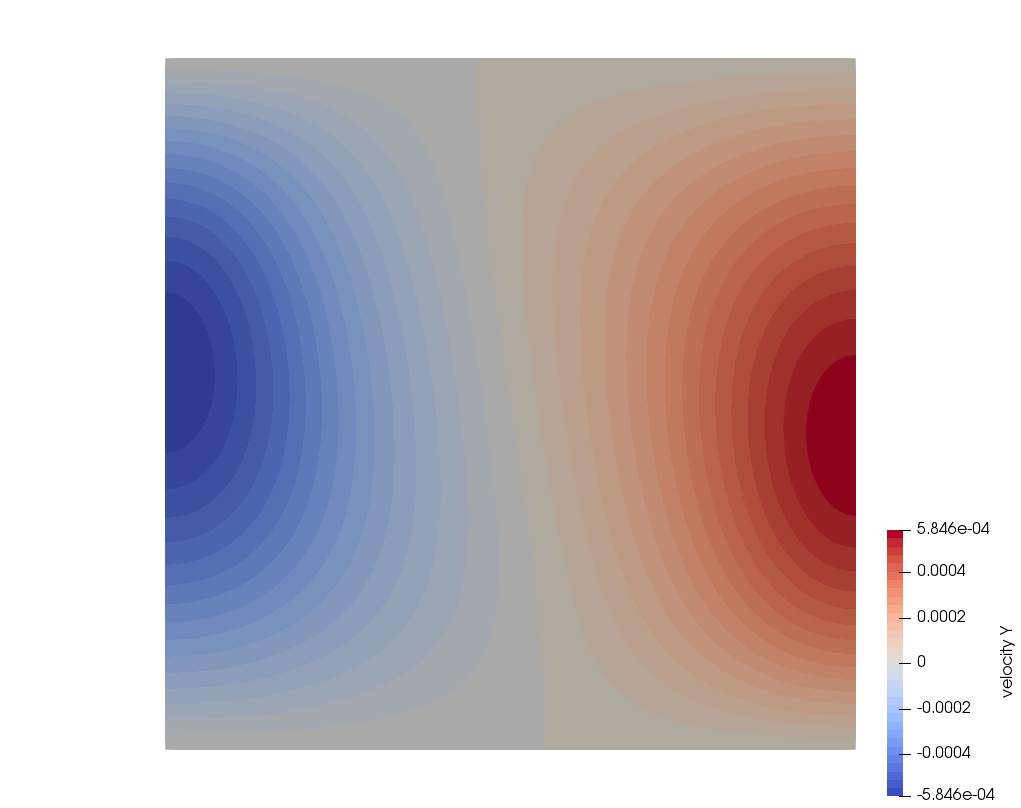
\includegraphics[width=4.5cm]{python_codes/fieldstone_24/BA_104/v.png}
(c)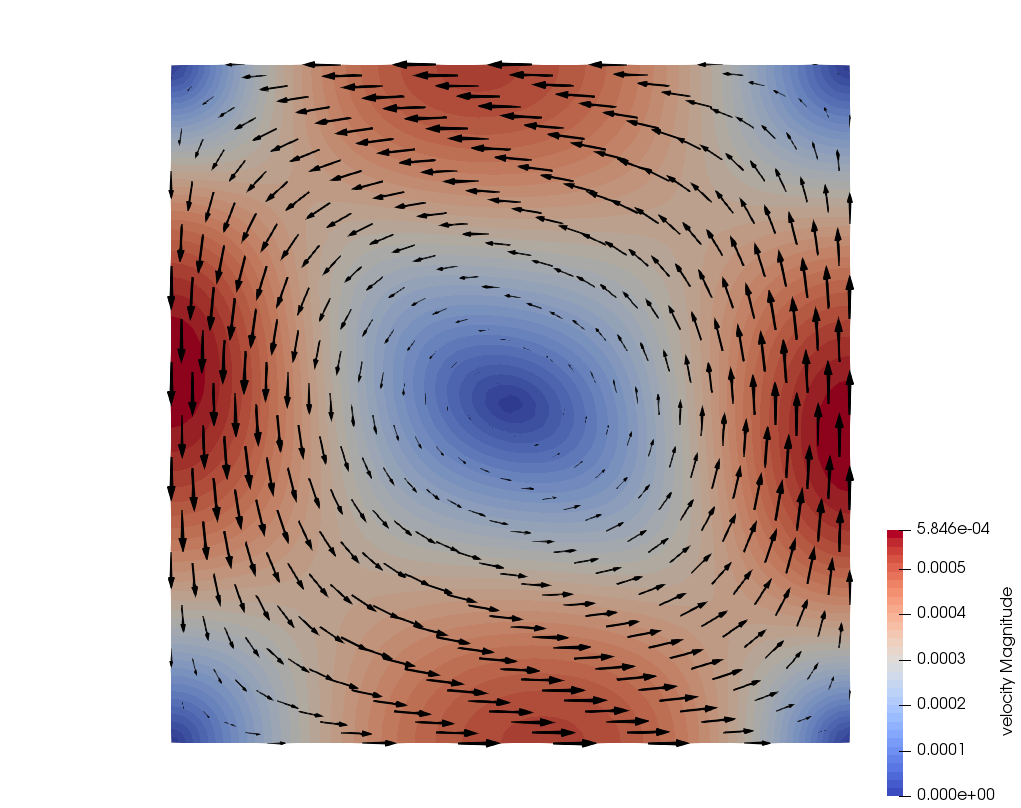
\includegraphics[width=4.5cm]{python_codes/fieldstone_24/BA_104/vel.png}\\
(d)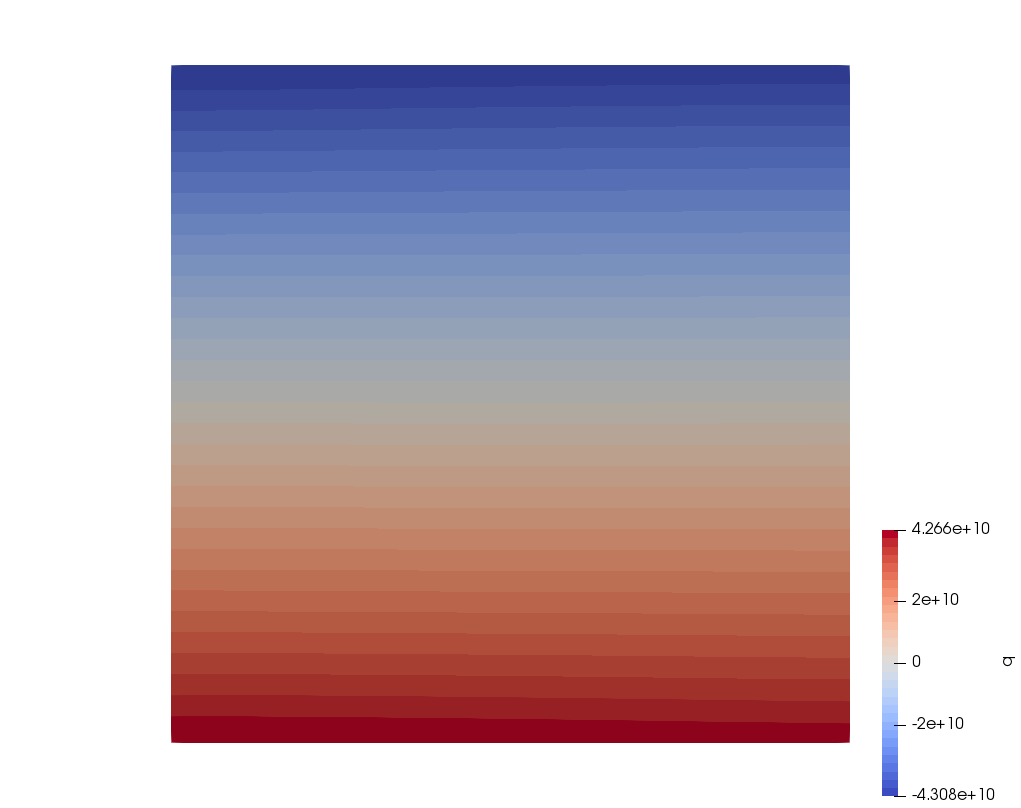
\includegraphics[width=4.5cm]{python_codes/fieldstone_24/BA_104/q.png}    
(e)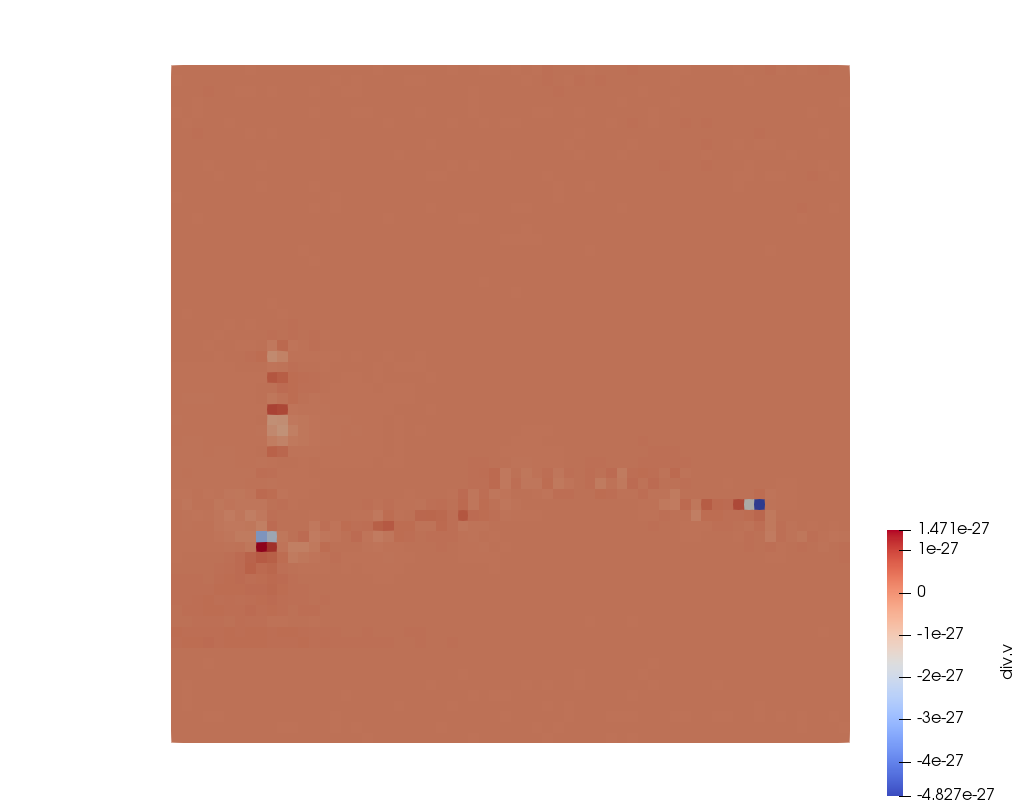
\includegraphics[width=4.5cm]{python_codes/fieldstone_24/BA_104/divv.png}    
(f)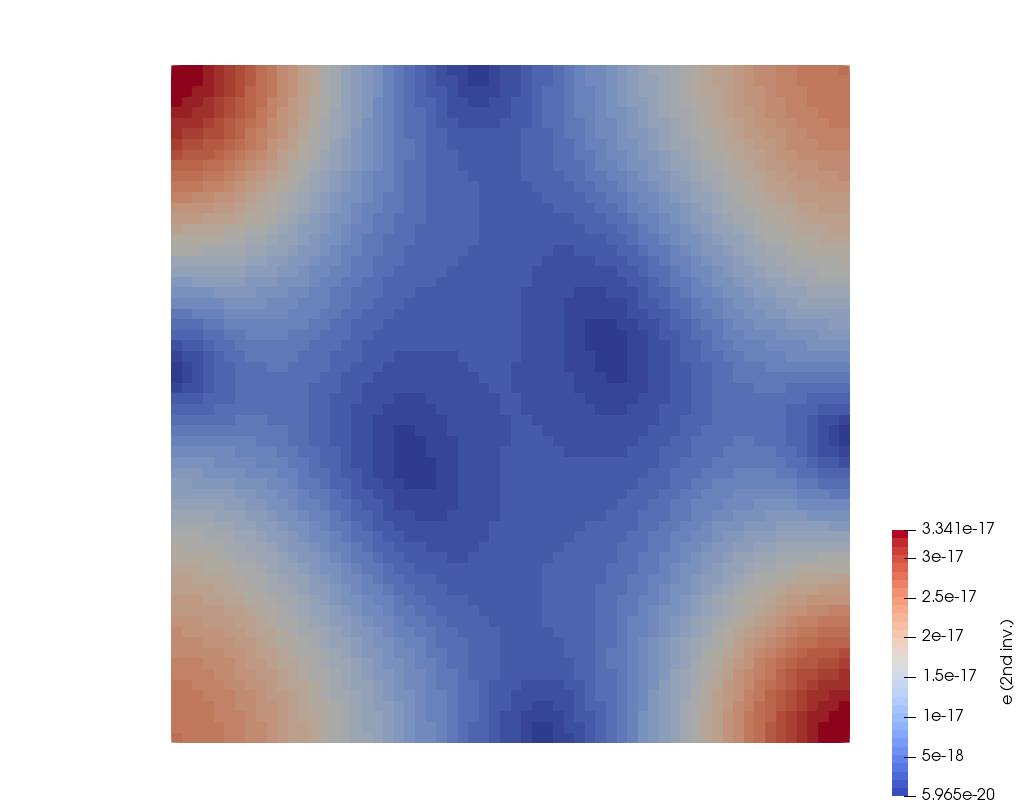
\includegraphics[width=4.5cm]{python_codes/fieldstone_24/BA_104/e2.png}   \\
(g)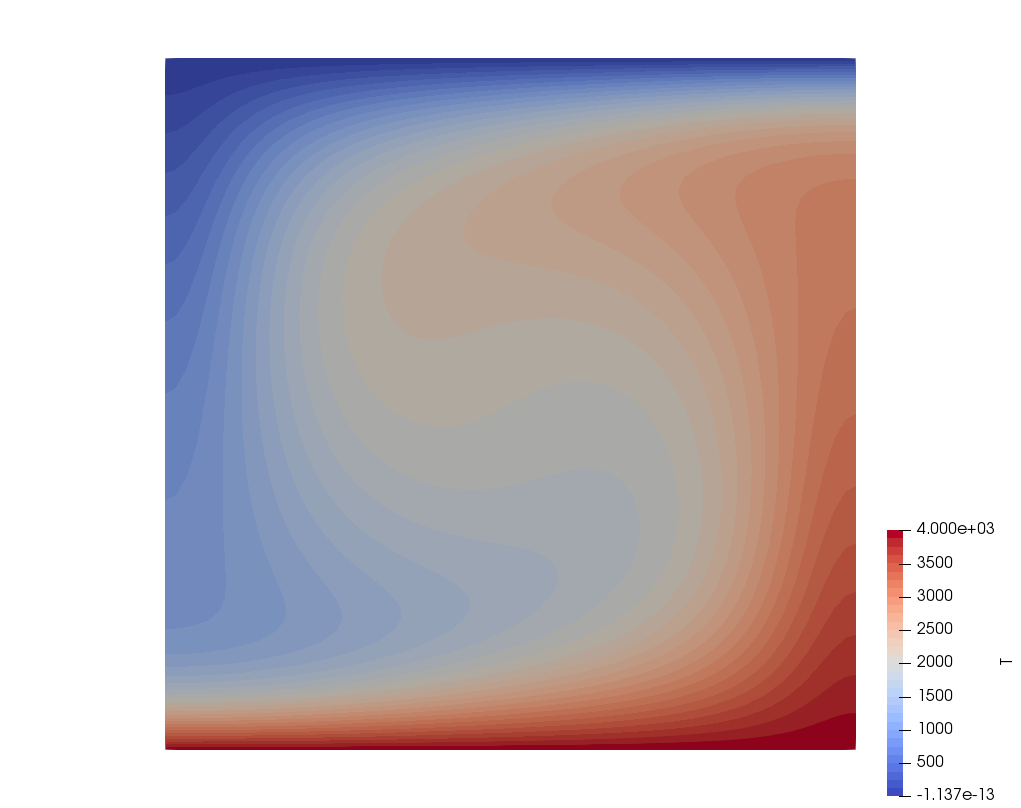
\includegraphics[width=4.5cm]{python_codes/fieldstone_24/BA_104/T.png} 
(h)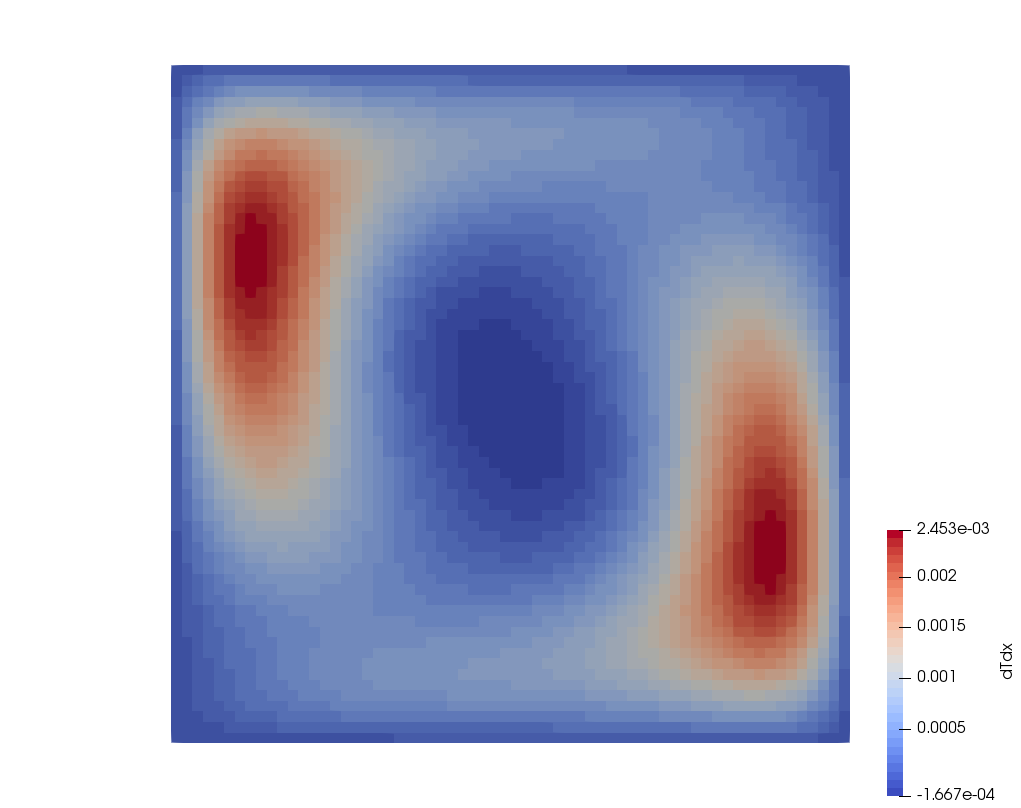
\includegraphics[width=4.5cm]{python_codes/fieldstone_24/BA_104/dTdx.png}
(i)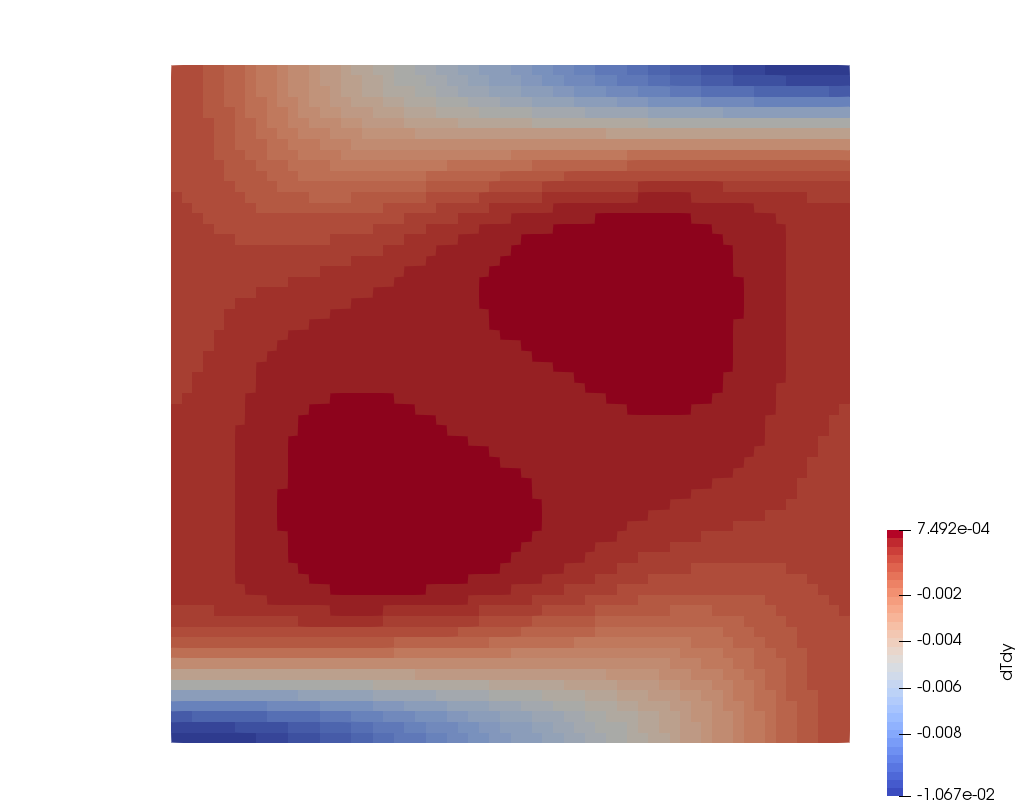
\includegraphics[width=4.5cm]{python_codes/fieldstone_24/BA_104/dTdy.png}  \\
\end{center}

\newpage
%-------------------------------------------------------
\subsection*{results - BA - $Ra=10^5$}

These results were obtained with a 64x64 resolution, and CFL number of 1. Steady state was reached 
after about 1250 timesteps.

\begin{center}
(a)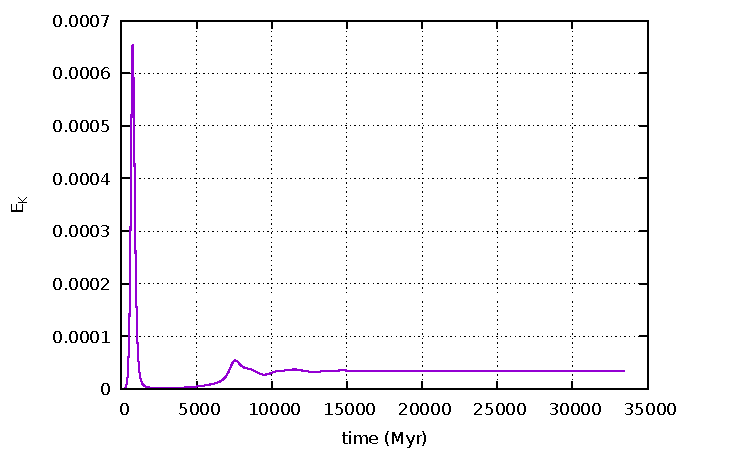
\includegraphics[width=4.5cm]{python_codes/fieldstone_24/BA_105/EK}
(b)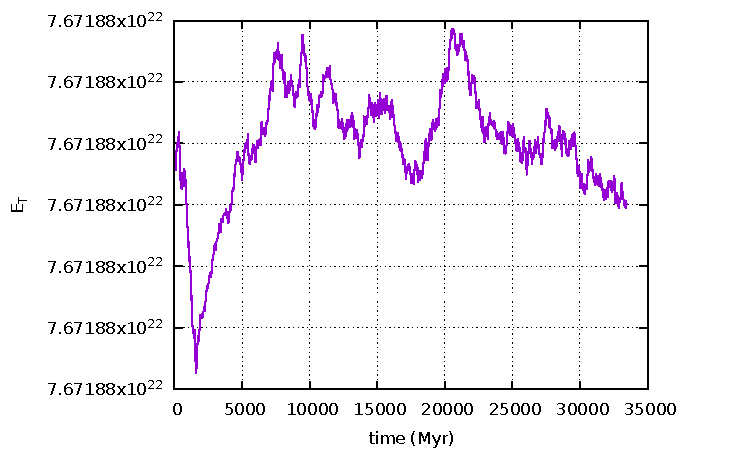
\includegraphics[width=4.5cm]{python_codes/fieldstone_24/BA_105/ET}
(c)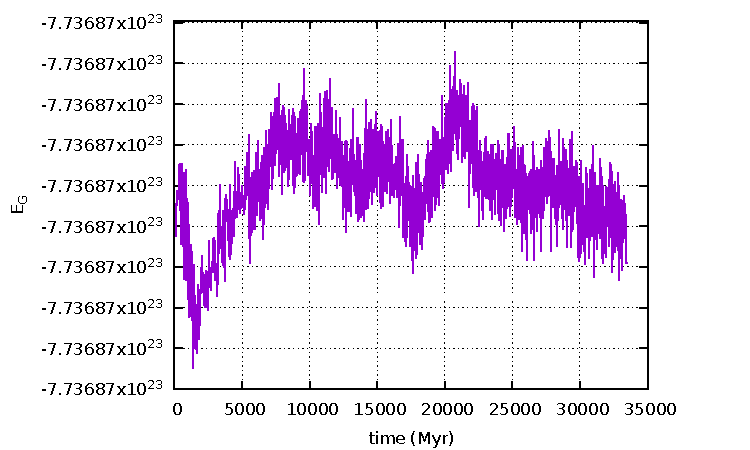
\includegraphics[width=4.5cm]{python_codes/fieldstone_24/BA_105/EG}\\
(d)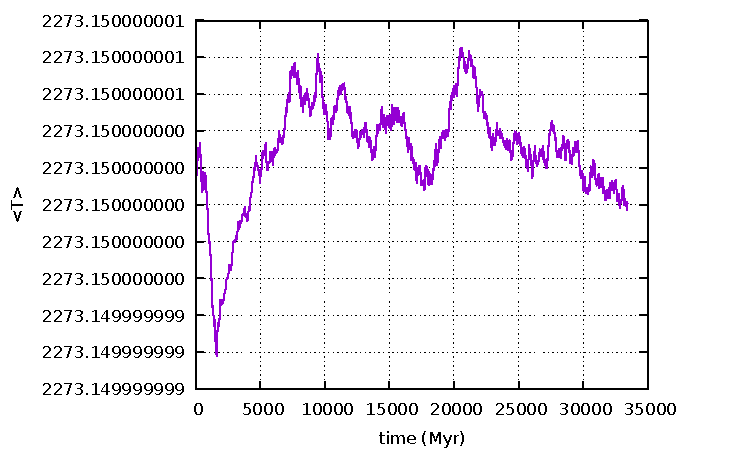
\includegraphics[width=4.5cm]{python_codes/fieldstone_24/BA_105/Tavrg}
(e)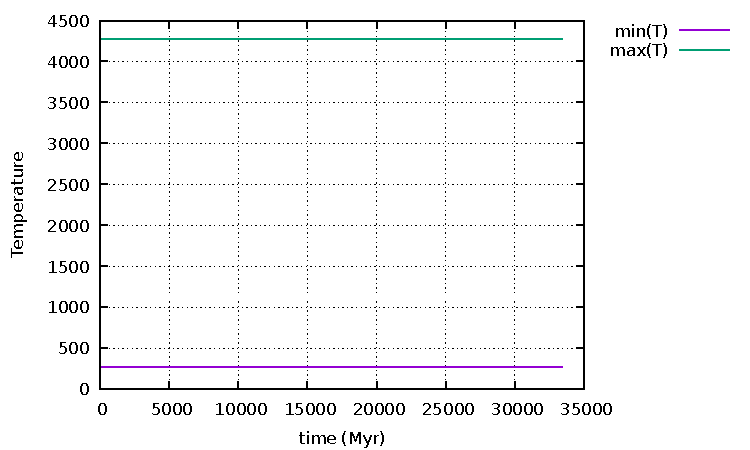
\includegraphics[width=4.5cm]{python_codes/fieldstone_24/BA_105/T_stats}
(f)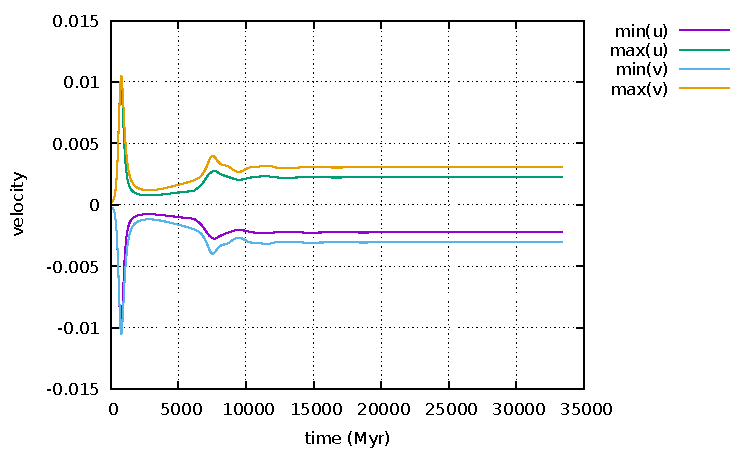
\includegraphics[width=4.5cm]{python_codes/fieldstone_24/BA_105/vel_stats}\\
(g)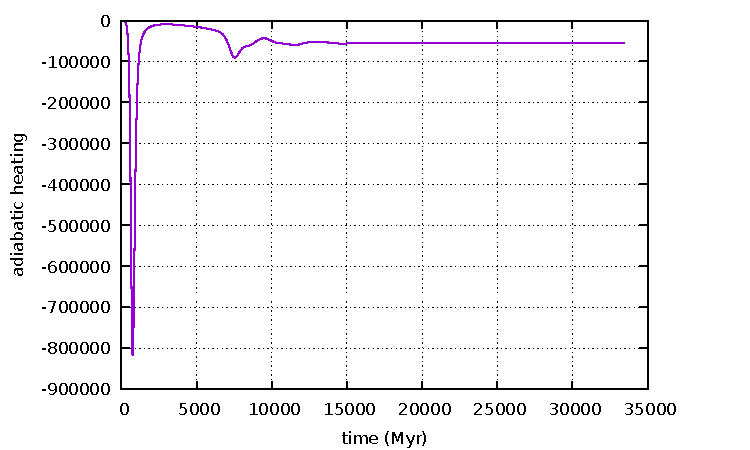
\includegraphics[width=4.5cm]{python_codes/fieldstone_24/BA_105/adiabatic_heating}
(h)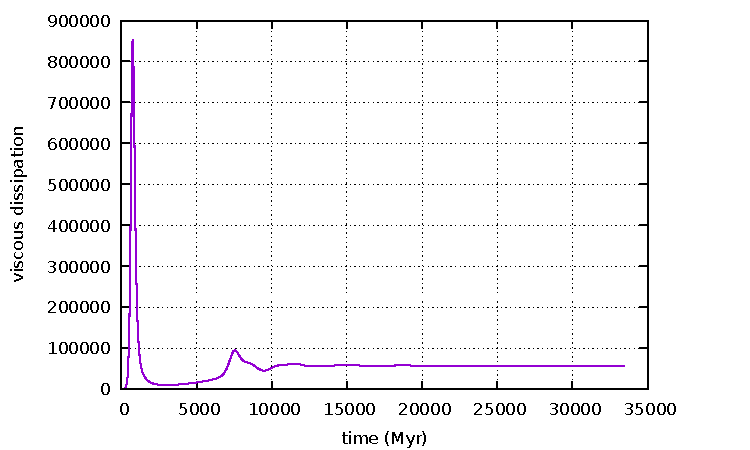
\includegraphics[width=4.5cm]{python_codes/fieldstone_24/BA_105/viscous_dissipation}
(i)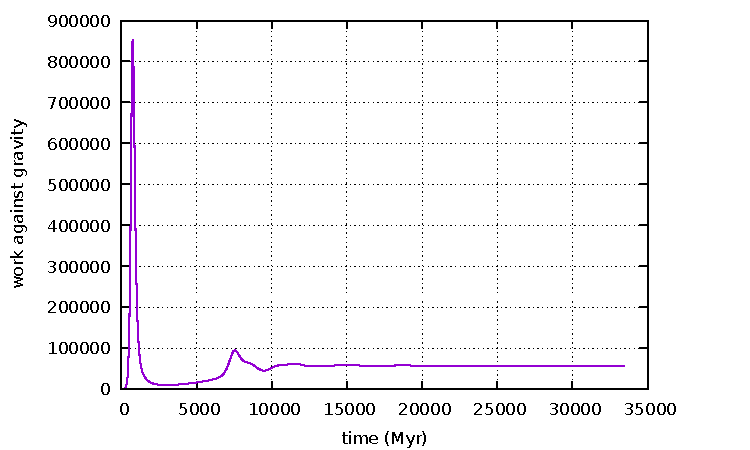
\includegraphics[width=4.5cm]{python_codes/fieldstone_24/BA_105/work_grav}\\
(j)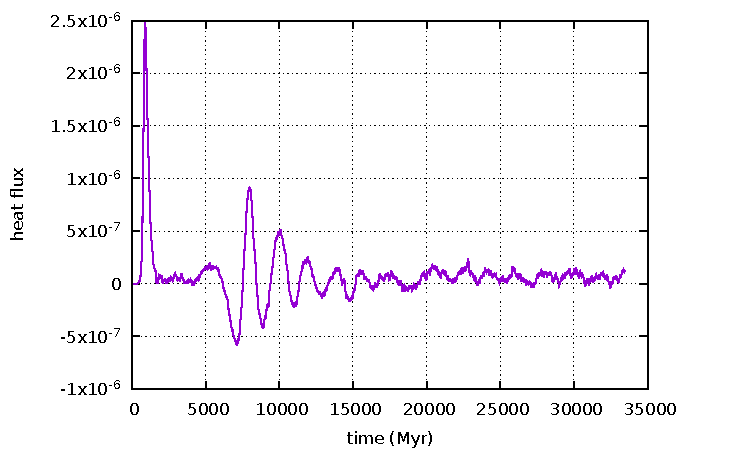
\includegraphics[width=4.5cm]{python_codes/fieldstone_24/BA_105/heat_flux}
(k)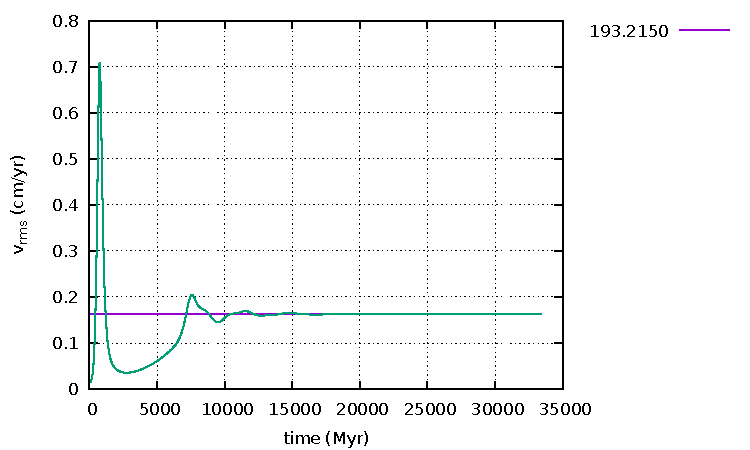
\includegraphics[width=4.5cm]{python_codes/fieldstone_24/BA_105/vrms}
(l)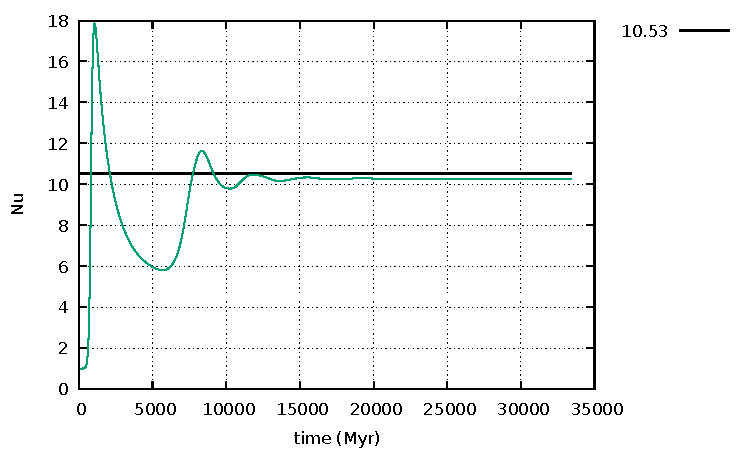
\includegraphics[width=4.5cm]{python_codes/fieldstone_24/BA_105/Nu}\\
(l)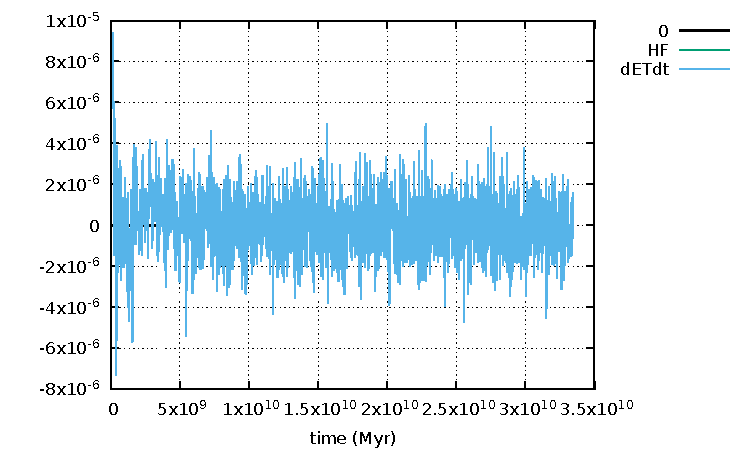
\includegraphics[width=7cm]{python_codes/fieldstone_24/BA_105/conservation1}
(m)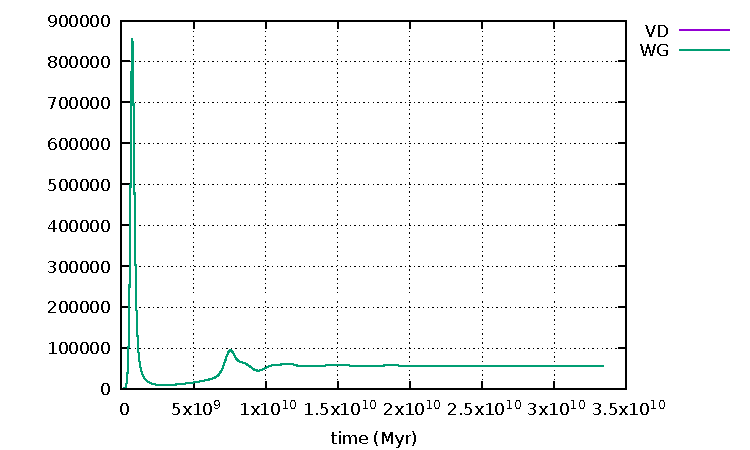
\includegraphics[width=7cm]{python_codes/fieldstone_24/BA_105/conservation2}\\
AH: adiabatic heating, VD: viscous dissipation, HF: heat flux, WG: work against gravity
\end{center}

Eq.(\ref{ba005}) is verified by (l) and Eq.(\ref{ba003}) is verified by (m).




\newpage
%-------------------------------------------------------
\subsection*{results - BA - $Ra=10^6$}






\newpage
%-------------------------------------------------------
\subsection*{results - EBA - $Ra=10^4$}

These results were obtained with a 64x64 resolution, and CFL number of 1. Steady state was reached 
after about 2500 timesteps 

\begin{center}
(a)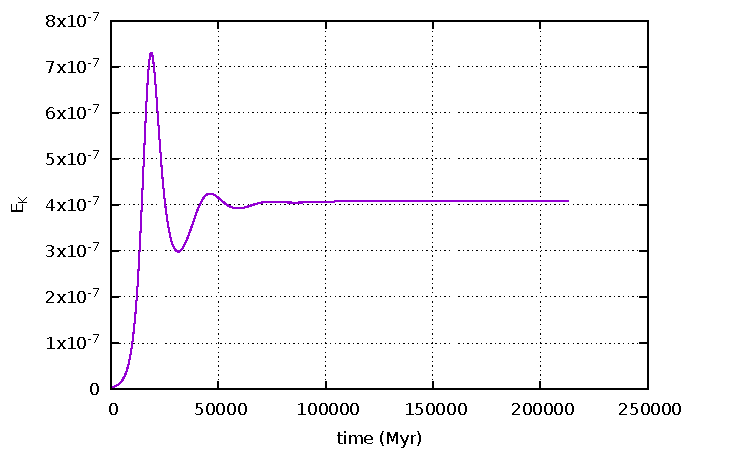
\includegraphics[width=4.5cm]{python_codes/fieldstone_24/EBA_104/EK}
(b)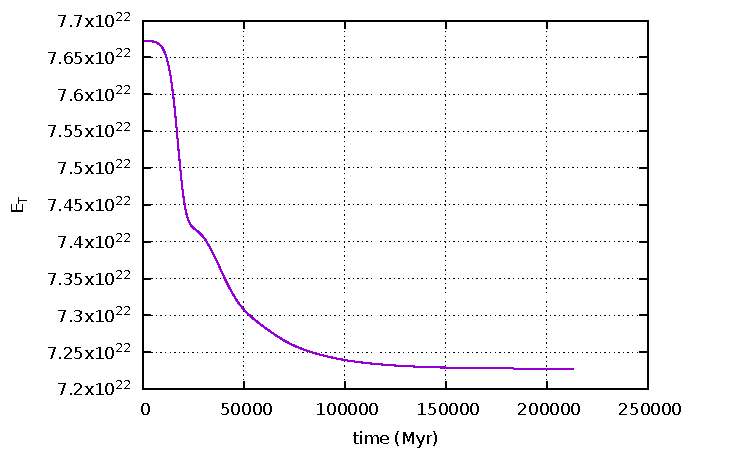
\includegraphics[width=4.5cm]{python_codes/fieldstone_24/EBA_104/ET}
(c)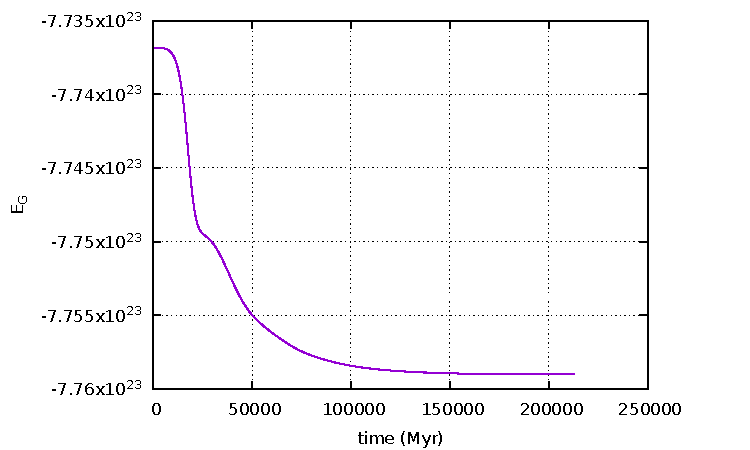
\includegraphics[width=4.5cm]{python_codes/fieldstone_24/EBA_104/EG}\\
(d)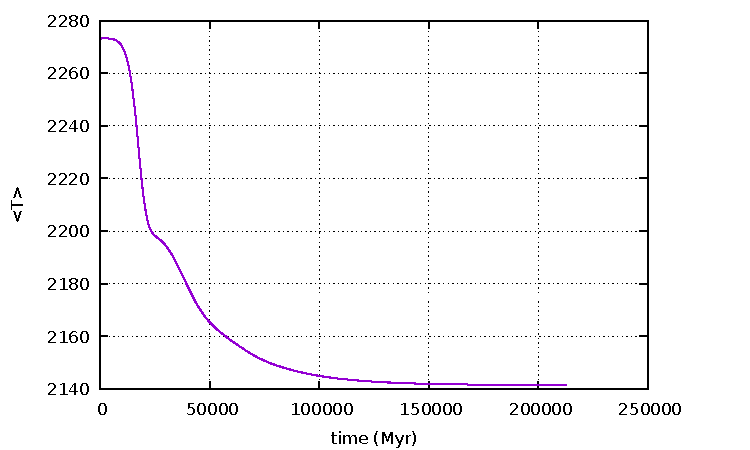
\includegraphics[width=4.5cm]{python_codes/fieldstone_24/EBA_104/Tavrg}
(e)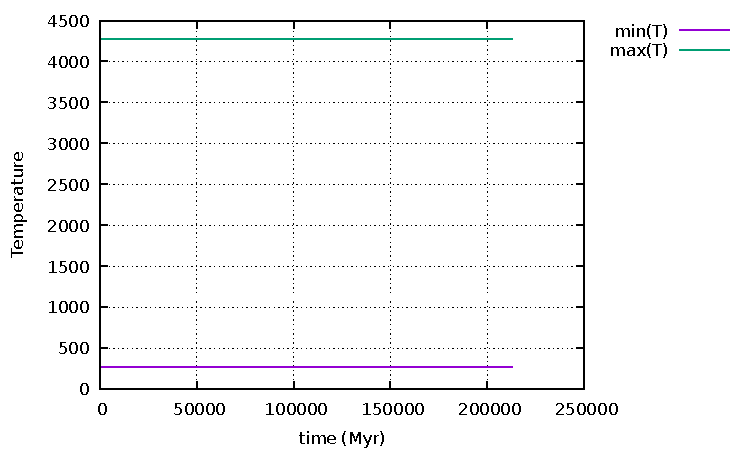
\includegraphics[width=4.5cm]{python_codes/fieldstone_24/EBA_104/T_stats}
(f)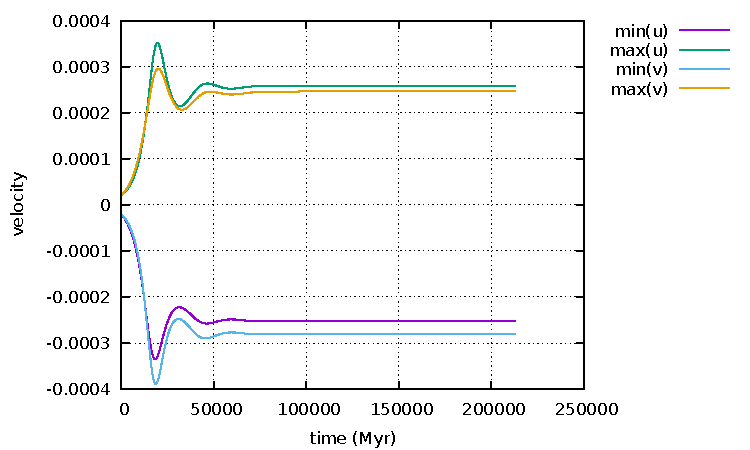
\includegraphics[width=4.5cm]{python_codes/fieldstone_24/EBA_104/vel_stats}\\
(g)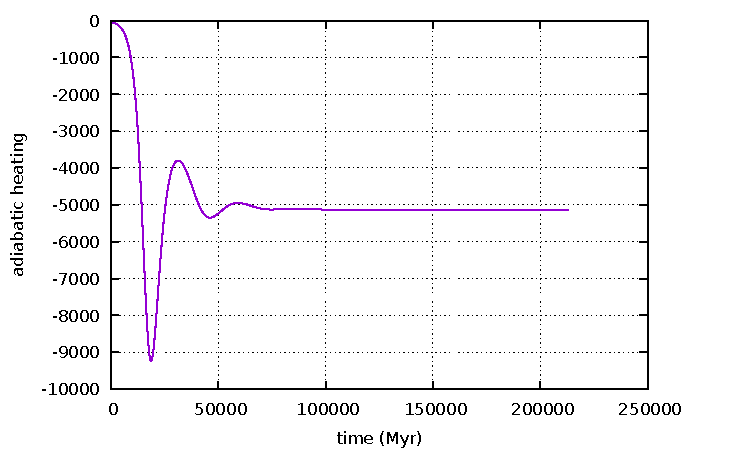
\includegraphics[width=4.5cm]{python_codes/fieldstone_24/EBA_104/adiabatic_heating}
(h)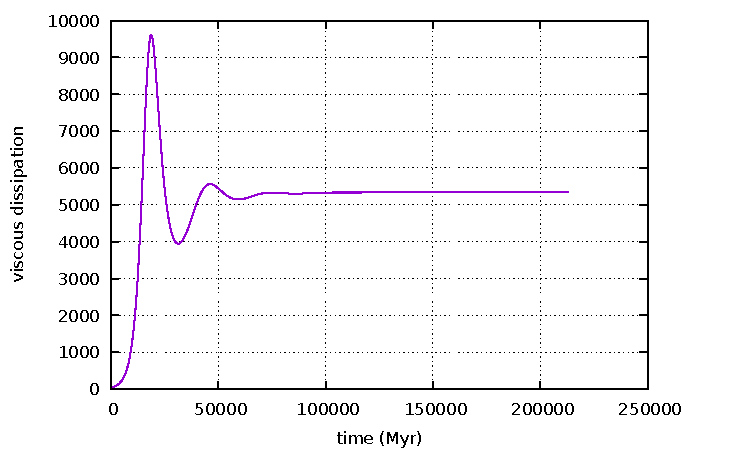
\includegraphics[width=4.5cm]{python_codes/fieldstone_24/EBA_104/viscous_dissipation}
(i)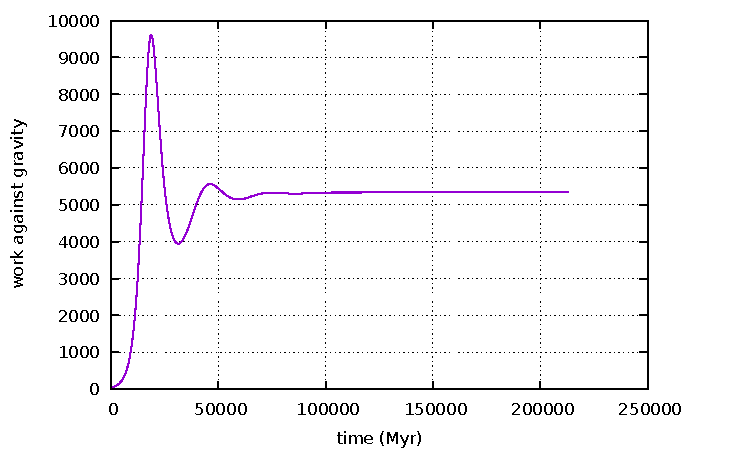
\includegraphics[width=4.5cm]{python_codes/fieldstone_24/EBA_104/work_grav}\\
(j)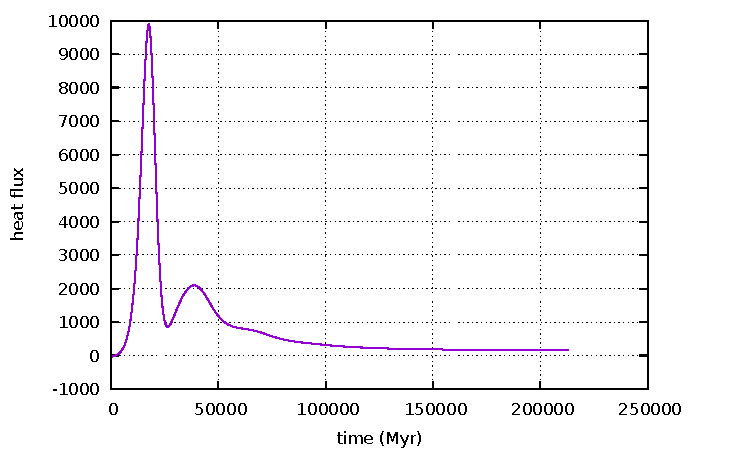
\includegraphics[width=4.5cm]{python_codes/fieldstone_24/EBA_104/heat_flux}
(k)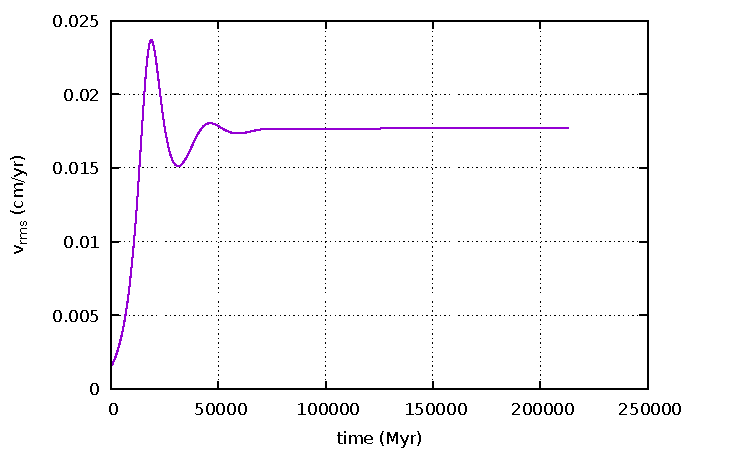
\includegraphics[width=4.5cm]{python_codes/fieldstone_24/EBA_104/vrms}
(l)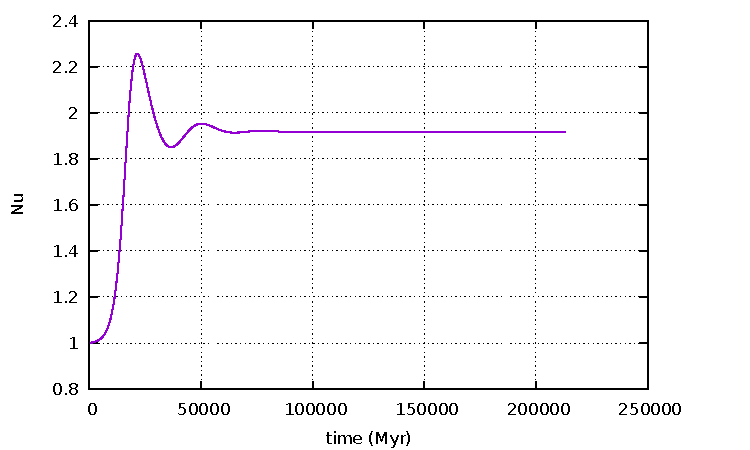
\includegraphics[width=4.5cm]{python_codes/fieldstone_24/EBA_104/Nu}\\
(l)\includegraphics[width=7cm]{python_codes/fieldstone_24/EBA_104/conservation1}
(m)\includegraphics[width=7cm]{python_codes/fieldstone_24/EBA_104/conservation2}\\
AH: adiabatic heating, VD: viscous dissipation, HF: heat flux, WG: work against gravity
\end{center}

Eq.(\ref{ba005}) is verified by (l) and Eq.(\ref{ba003}) is verified by (m).

\newpage
\begin{center}
a)\includegraphics[width=4.5cm]{python_codes/fieldstone_24/EBA_104/u.png}
b)\includegraphics[width=4.5cm]{python_codes/fieldstone_24/EBA_104/v.png}
c)\includegraphics[width=4.5cm]{python_codes/fieldstone_24/EBA_104/vel.png}\\
d)\includegraphics[width=4.5cm]{python_codes/fieldstone_24/EBA_104/q.png}    
e)\includegraphics[width=4.5cm]{python_codes/fieldstone_24/EBA_104/divv.png}    
f)\includegraphics[width=4.5cm]{python_codes/fieldstone_24/EBA_104/e2.png}   \\
g)\includegraphics[width=4.5cm]{python_codes/fieldstone_24/EBA_104/rho.png}  
h)\includegraphics[width=4.5cm]{python_codes/fieldstone_24/EBA_104/drhodx.png}  
i)\includegraphics[width=4.5cm]{python_codes/fieldstone_24/EBA_104/drhody.png} \\ 
j)\includegraphics[width=4.5cm]{python_codes/fieldstone_24/EBA_104/T.png} 
k)\includegraphics[width=4.5cm]{python_codes/fieldstone_24/EBA_104/dTdx.png}
l)\includegraphics[width=4.5cm]{python_codes/fieldstone_24/EBA_104/dTdy.png}  \\
m)\includegraphics[width=4.5cm]{python_codes/fieldstone_24/EBA_104/alpha_T_v_gradp.png}  
n)\includegraphics[width=4.5cm]{python_codes/fieldstone_24/EBA_104/Phi.png}
\end{center}



\newpage
%-------------------------------------------------------
\subsection*{results - EBA - $Ra=10^5$}

These results were obtained with a 64x64 resolution, and CFL number of 1. Simulation 
 was stopped after about 4300 timesteps. 

\begin{center}
(a)\includegraphics[width=4.5cm]{python_codes/fieldstone_24/EBA_105/EK}
(b)\includegraphics[width=4.5cm]{python_codes/fieldstone_24/EBA_105/ET}
(c)\includegraphics[width=4.5cm]{python_codes/fieldstone_24/EBA_105/EG}\\
(d)\includegraphics[width=4.5cm]{python_codes/fieldstone_24/EBA_105/Tavrg}
(e)\includegraphics[width=4.5cm]{python_codes/fieldstone_24/EBA_105/T_stats}
(f)\includegraphics[width=4.5cm]{python_codes/fieldstone_24/EBA_105/vel_stats}\\
(g)\includegraphics[width=4.5cm]{python_codes/fieldstone_24/EBA_105/adiabatic_heating}
(h)\includegraphics[width=4.5cm]{python_codes/fieldstone_24/EBA_105/viscous_dissipation}
(i)\includegraphics[width=4.5cm]{python_codes/fieldstone_24/EBA_105/work_grav}\\
(j)\includegraphics[width=4.5cm]{python_codes/fieldstone_24/EBA_105/heat_flux}
(k)\includegraphics[width=4.5cm]{python_codes/fieldstone_24/EBA_105/vrms}
(l)\includegraphics[width=4.5cm]{python_codes/fieldstone_24/EBA_105/Nu}\\
(l)\includegraphics[width=7cm]{python_codes/fieldstone_24/EBA_105/conservation1}
(m)\includegraphics[width=7cm]{python_codes/fieldstone_24/EBA_105/conservation2}\\
AH: adiabatic heating, VD: viscous dissipation, HF: heat flux, WG: work against gravity
\end{center}


\newpage
\subsection*{Onset of convection}

The code can be run for values of Ra between 500 and 1000, at various resolutions for the BA formulation.
The value $v_{rms}(t)-v_{rms}(0)$ is plotted as a function of $Ra$ and for the 10 first timesteps. If the $v_{rms}$
is found to decrease, then the Rayleigh number is not high enough to allow for convection and the initial temperature
perturbation relaxes by diffusion (and then $v_{rms}(t)-v_{rms}(0)<0$. If the $v_{rms}$ is found to increase, then 
$v_{rms}(t)-v_{rms}(0)>0$ and the system is going to showcase convection. The zero value of $v_{rms}(t)-v_{rms}(0)$ 
gives us the critical Rayleigh number, which is found between 775 and 790. 


\begin{center}
\includegraphics[width=8cm]{python_codes/fieldstone_24/ONSET/onset.pdf} 
\includegraphics[width=8cm]{python_codes/fieldstone_24/ONSET/onset_zoom.pdf}
\end{center}

\newpage
{\bf Appendix}: Looking for the right combination of parameters for the King benchmark.

I run a quadruple do loop over $L$, $\Delta T$, $\rho_0$ and $\eta_0$ between plausible values 
(see code targets.py) and write in a file only the combination which yields the 
required Rayleigh and Dissipation number values (down to 1\% accuracy).

\begin{lstlisting}
alpha=3e-5
g=10
hcapa=1250
hcond=3
DTmin=1000  ; DTmax=4000  ; DTnpts=251
Lmin=1e6    ; Lmax=3e6    ; Lnpts=251
rhomin=3000 ; rhomax=3500 ; rhonpts=41
etamin=19   ; etamax=25   ; etanpts=100
\end{lstlisting}


On the following plots the 'winning' combinations of these four parameters are shown:
\begin{center}
\includegraphics[width=8cm]{python_codes/fieldstone_24/looking_for_Ra_Di/RaDi.pdf}
\includegraphics[width=8cm]{python_codes/fieldstone_24/looking_for_Ra_Di/DTL.pdf}
\includegraphics[width=8cm]{python_codes/fieldstone_24/looking_for_Ra_Di/rhoeta.pdf}
\end{center}

We see that:
\begin{itemize}
\item the parameter $L$ (being to the 3rd power in the $Ra$ number) cannot vary too much. Although it is 
varied between 1000 and 3000km there seems to be a 'right' value at about 1040 km. (why?)
\item viscosities are within $10^{23}$ and $10^{24}$ which are plausible values (although a bit high?).
\item densities can be chosen freely between 3000 and 3500
\item $\Delta T$ seems to be the most problematic value since it can range from 1000 to 4000K ...  
\end{itemize}


